%
% Zusammenfassung Communication Networks D-ITET
% ===========================================================================
% Author:			Marco Dober
% Version:			0.1
% Last changed: 	19.02.2019	
% ---------------------------------------------------------------------------

\documentclass[a4paper, fontsize=8pt, landscape, DIV=1]{scrartcl}
\usepackage{lastpage}
\usepackage{hyperref}
\usepackage[graphicx]{realboxes}
% Include general settings and customized commands
%
% General packages and settings
% ===========================================================================
% Author:			Silvano Cortesi (cortesis@student.ethz.ch)
% Version:			1.2
% Last changed:		03.01.2018
%
% ---------------------------------------------------------------------------




\usepackage[german]{babel} %choose your language \usepackage[german]{babel}
%\usepackage[T1]{fontenc}
\usepackage[utf8]{inputenc}
\usepackage{fancyhdr}
%\usepackage{lastpage}
%\usepackage{lmodern}
\usepackage{enumerate}
%\usepackage{float} % for positioning of figures
\usepackage[landscape, margin=1cm]{geometry}
\usepackage[dvipsnames]{xcolor}
\usepackage{pdfpages}


%% Math %%
\usepackage{todonotes}
\usepackage{amscd}
\usepackage{blindtext}
\usepackage{enumitem}
\usepackage{multicol}
\usepackage{parskip}
\usepackage{empheq}
\usepackage{amsmath}
\usepackage{amsfonts}
\usepackage{amssymb}
\usepackage{amsthm}
%\usepackage{dsfont}
%\usepackage{esint} % provides \oiint
\usepackage{mathrsfs}
%\usepackage{trfsigns}
%\numberwithin{equation}{subsection}
%\usepackage{numprint}

%% Graphics & Charts %%
\usepackage{graphicx}
%\usepackage{pdfpages}
%\usepackage{booktabs}
\usepackage{array}
%\usepackage{paralist}
%\usepackage{framed}
%\usepackage{trfsigns}
\usepackage{tikz}
%\usepackage[lofdepth,lotdepth]{subfig}
%\usepackage{tikz}  %Graphen zeichnen
%\usetikzlibrary{decorations.pathmorphing}
%\usetikzlibrary{arrows.meta,arrows}
%\usepackage{pgfplots}
%% General Settings %%
%\setlength{\parindent}{0px}
%\setkomafont{captionlabel}{\normalfont\bfseries}

%\pagestyle{fancy}
%\lfoot{\tiny \today}
%\rfoot{\thepage\  / \pageref{LastPage}}
%\cfoot{}
%\renewcommand{\footrulewidth}{0.4pt}

%% provides command \uline{} for underlining words
%\usepackage{ulem}

%% colour headings
%\usepackage{color}
%\definecolor{bluen}{cmyk}{1,0.5,0,0}
%\definecolor{bloodorange}{cmyk}{0,.92,1,.2}
%\addtokomafont{section}{\color{bloodorange}}
%\addtokomafont{subsection}{\color{bloodorange}}
%\addtokomafont{subsubsection}{\color{bloodorange}}
%\addtokomafont{paragraph}{\small\color{bloodorange}}
%\addtokomafont{subparagraph}{\small\color{bloodorange}}

%% Signs & Special Formating %%
%\usepackage{ulem} %normalem: \emph{Text} is italic again.
%\usepackage{multicol,multirow}
%\usepackage{tabularx}
%\usepackage{stackrel}
%\usepackage{makeidx}
%\usepackage{mparhack} % bessere margiale bei seitenumbruch

% make document compact
\usepackage[compact]{titlesec}
\titlespacing{\section}{0pt}{*0}{*0}
\titlespacing{\subsection}{0pt}{*0}{*0}
\titlespacing{\subsubsection}{0pt}{*0}{*0}

\parindent 0pt
\pagestyle{empty}
\setlength{\unitlength}{1cm}
\setlist{leftmargin = *}

%include also newer PDF
\pdfminorversion=6

% Set the color of your style
% Avaiable are: Apricot, Aquamarine, Bittersweet, Black, Blue, blue, BlueGreen, BlueViolet, BrickRed, Brown, BurntOrange, CadetBlue, CarnationPink, Cerulean, CornflowerBlue, Cyan, Dandelion, DarkOrchid, Emerald, ForestGreen, Fuchsia, Goldenrod, Gray, Green, GreenYellow, JungleGreen, Lavender, ... (more at: http://en.wikibooks.org/wiki/LaTeX/Colors)
\def\StyleColor{MidnightBlue}

%
% General commands
% ===========================================================================
% Author:			Silvano Cortesi (cortesis@student.ethz.ch)
% Version:			1.2
% Last changed:		03.01.2018
%
% ---------------------------------------------------------------------------

%..ROEMISCHE_ZAHLEN
	\newcommand{\Roe}[1]{\uppercase\expandafter{\romannumeral #1 }}

%..ZAHLENMENGEN
	\newcommand{\N}{\mathbb{N}}
	\newcommand{\Z}{\mathbb{Z}}
	\newcommand{\Q}{\mathbb{Q}}
	\newcommand{\R}{\mathbb{R}}
	\newcommand{\real}{\R}
	\newcommand{\C}{\mathbb{C}}
	\newcommand{\complex}{\C}
	\newcommand{\0}{\mathbb{O}}
	\newcommand{\F}{\mathbb{F}}
	\newcommand{\K}{\mathbb{K}}
    \newcommand{\angstrom}{\textup{\AA}}
    
%..PFEILE
	\renewcommand{\leadsto}{\Longrightarrow}
	\newcommand{\leftrightleadsto}{\Longleftrightarrow}

%..VEKTOREN
	\newcommand{\Ul} {\underline}
	\newcommand{\vEx} {\vec{e}_x}
	\newcommand{\vEy} {\vec{e}_y}
	\newcommand{\vEz} {\vec{e}_z}
	\newcommand{\vEq} {\vec{e_1}}
	\newcommand{\vEw} {\vec{e_2}}
	\newcommand{\vEe} {\vec{e_3}}
	\newcommand{\transpose} {^{\text{T}}}
	\newcommand{\vect}[1]{\boldsymbol{#1}}
	
%..MATRIX
    \newcommand{\MATR}[1]{ \displaystyle \left( \begin{matrix} #1 \end{matrix} \right)}
    \newcommand{\MATRABS}[1]{ \displaystyle \left| \begin{matrix} #1 \end{matrix} \right|}

%..GRAPHICS
  \newcommand{\cgraphic}[2]{\begin{center}\includegraphics[width=#1\columnwidth,keepaspectratio]{#2}\end{center}}
  
%..FONTS AND LETTERS
  \newcommand*{\rom}[1]{\uppercase\expandafter{\romannumeral #1\relax}}

%..KOMPLEXE ZAHLEN
	\renewcommand{\Re}{\text{Re}\,}
	\renewcommand{\Im}{\text{Im}\,}

%..OPERATOREN
	\DeclareMathOperator{\grad}{grad}
	\renewcommand{\div}{\text{div}\,}
    	\DeclareMathOperator{\rot}{rot}
    	\DeclareMathOperator{\divg}{div}
    	\DeclareMathOperator{\Tr}{Tr}
    	\DeclareMathOperator{\const}{const}
	\DeclareMathOperator{\imag}{i}
	\newcommand{\Lapl}{\hbox{\footnotesize{$\Delta$}}}

%..DIFFERENTIALRECHNUNG
	\newcommand{\Dx} {\,\mathrm{d}}
	\newcommand{\abl}[1] {\frac{\mathrm{d}}{\mathrm{d}#1}}
	\newcommand{\Abl}[2] {\frac{\mathrm{d}#1}{\mathrm{d}#2}}
	\newcommand{\ablq}[1] {\frac{\mathrm{d^2}}{\mathrm{d}#1^2}}
	\newcommand{\Ablq}[2] {\frac{\mathrm{d^2}#1}{\mathrm{d}#2^2}}
	\newcommand{\pabl}[1] {\frac{\partial}{\partial#1}}
	\newcommand{\pablq}[1] {\frac{\partial^2}{\partial#1^2}}
	\newcommand{\Pabl}[2] {\frac{\partial#1}{\partial#2}}
	\newcommand{\Pablq}[2] {\frac{\partial^2#1}{\partial#2^2}}

%..INTEGRALRECHNUNG
	\newcommand{\dint}{\displaystyle{\int}}
	\newcommand{\intab}{\int^b_a}
	\newcommand{\intinf}{\int_{-\infty}^\infty}
	\newcommand{\dintab}{\displaystyle{\int^b_a}}
	\newcommand{\dintpi}{\displaystyle{\int^{\pi}_{-\pi}}}
	\newcommand{\dintzpi}{\displaystyle{\int^{2\pi}_{\mbox{-}2\pi}}}
	\newcommand{\dA}{\hspace{4pt}\mathrm{d}A}
	\newcommand{\dx}{\hspace{4pt}\mathrm{d}x}
	\newcommand{\dy}{\hspace{4pt}\mathrm{d}y}
	\newcommand{\dz}{\hspace{4pt}\mathrm{d}z}
	\newcommand{\dr}{\hspace{4pt}\mathrm{d}r}
	\newcommand{\ds}{\hspace{4pt}\mathrm{d}s}
	\newcommand{\dS}{\hspace{4pt}\mathrm{d}S}
	\newcommand{\dt}{\hspace{4pt}\mathrm{d}t}
	\newcommand{\dm}{\hspace{4pt}\mathrm{d}m}
	\newcommand{\dk}{\hspace{4pt}\mathrm{d}k}
	\newcommand{\dl}{\hspace{4pt}\mathrm{d}l}
	\newcommand{\du}{\hspace{4pt}\mathrm{d}u}
	\newcommand{\dv}{\hspace{4pt}\mathrm{d}v}
	\newcommand{\dV}{\hspace{4pt}\mathrm{d}V}
	\newcommand{\dphi}{\hspace{4pt}\mathrm{d}\varphi}
	\newcommand{\domega}{\hspace{4pt}\mathrm{d}\omega}
	\newcommand{\dvarsigma}{\hspace{4pt}\mathrm{d}\varsigma}
	\newcommand{\dtau}{\hspace{4pt}\mathrm{d}\tau}
	\newcommand{\dtheta}{\hspace{4pt}\mathrm{d}\vartheta}
	\newcommand{\dmu}{\hspace{4pt}\mathrm{d}\mu}
	\newcommand{\dxi}{\hspace{4pt}\mathrm{d}\xi}
	\newcommand{\deta}{\hspace{4pt}\mathrm{d}\eta}
	\newcommand{\dvecl}{\hspace{4pt}\mathrm{d}\vec{l}}
	\newcommand{\dvecS}{\hspace{4pt}\mathrm{d}\vec{S}}

%..LIMES
    \DeclareMathOperator{\limni}{\lim\limits_{n\to\infty}}
    \DeclareMathOperator{\limxi}{\lim\limits_{x\to\infty}}
    \DeclareMathOperator{\limho}{\lim\limits_{h\to0}}
    \newcommand{\limxai}[1]{\ensuremath{\lim\limits_{x\to #1}}}

%..SUMMEN
    \DeclareMathOperator{\sumni}{\sum_{n=0}^{\infty}}
    \newcommand{\sumnia}[1]{\ensuremath{\sum_{n=#1}^{\infty}}}


%..PARTIELLE ABLEITUNG
    \DeclareMathOperator{\partf}{\dfrac{\partial f}{\partial x}}
    \newcommand{\partfo}[1]{\ensuremath{\dfrac{\partial f}{\partial #1}}}
    \newcommand{\parto}[1]{\ensuremath{\dfrac{\partial }{\partial #1}}}
    \newcommand{\partt}[2]{\ensuremath{\dfrac{\partial^2 }{\partial #1\partial #2}}}
    \newcommand{\partq}[1]{\ensuremath{\dfrac{\partial^2 }{\partial #1^2}}}


%..ENUMERATION
    \newenvironment{abc}{\begin{enumerate}[(a)]}{\end{enumerate}}
    \newenvironment{cabc}{\begin{compactenum}[(a)]}{\end{compactenum}}
    \newenvironment{romanenum}{\begin{enumerate}[i.]}{\end{enumerate}}
    \newenvironment{cromanenum}{\begin{compactenum}[i.]}{\end{compactenum}}

%..FUNCTIONS
    \DeclareMathOperator{\arsinh}{arsinh}
    \DeclareMathOperator{\arcosh}{arcosh}
    \DeclareMathOperator{\artanh}{artanh}
    \DeclareMathOperator{\arcoth}{arcoth}
    \DeclareMathOperator{\arccot}{arccot}
    \DeclareMathOperator{\Arg}{Arg}
    \DeclareMathOperator{\Log}{Log}
    \newcommand{\dis}[1]{\hspace{#1cm}}
    \newcommand{\abs}[1]{\ensuremath{\left\vert#1\right\vert}}
    \newcommand{\attention}{\raisebox{-1pt}{{\makebox[1.6em][c]{\makebox[0pt][c]{\raisebox{.13em}{\small!}}\makebox[0pt][c]{\color{red}\Large$\bigtriangleup$}}}}}
    \DeclareMathOperator{\meq}{\stackrel{!}{=}}
    
    
% section color box
\setkomafont{section}{\mysection}
\newcommand{\mysection}[1]{%
    \Large\sffamily\bfseries%
    \setlength{\fboxsep}{0cm}%already boxed
    \colorbox{\StyleColor!40}{%
        \begin{minipage}{\linewidth}%
            \vspace*{2pt}%Space before
            #1
            \vspace*{-1pt}%Space after
        \end{minipage}%
    }}

%subsection color box
\setkomafont{subsection}{\mysubsection}
\newcommand{\mysubsection}[1]{%
    \normalsize \sffamily\bfseries%
    \setlength{\fboxsep}{0cm}%already boxed
    \colorbox{\StyleColor!20}{%
        \begin{minipage}{\linewidth}%
            \vspace*{2pt}%Space before
             #1
            \vspace*{-1pt}%Space after
        \end{minipage}%
    }}

% highlighter
\newcommand{\hilight}[1]{\colorbox{\StyleColor}{#1}}
\newcommand{\highlighty}[1]{%
  \setlength{\fboxsep}{0pt}\colorbox{yellow!100}{\ensuremath{#1}}}

\newcommand{\highlightg}[1]{%
  \setlength{\fboxsep}{0pt}\colorbox{green!100}{\ensuremath{#1}}}

\newcommand{\highlightbg}[1]{%
   \colorbox{green!100}{$\displaystyle #1$}}  

% equation box        
\newcommand{\eqbox}[1]{\setlength{\fboxrule}{1mm}\fcolorbox{\StyleColor}{white}{\hspace{0.5em}$\displaystyle#1$\hspace{0.5em}}}

%center equationbox
\newcommand{\ceqbox}[1]{\vspace*{4pt} \begin{center}\eqbox{#1}\end{center}\vspace*{4pt}}

%change page style for header
\pagestyle{fancy}
\footskip 20pt
\rhead{Marco Dober}
\lhead{Communication Networks}
\chead{\thepage}
\cfoot{}
\headheight 17pt \headsep 10pt
\title{Communication Networks}
\author{Marco Dober}
\date{\today}


\begin{document}
	\setcounter{secnumdepth}{3} %no enumeration of sections
	\begin{multicols*}{4}
		%
		\section*{Disclaimer}
			This should be a summary of the Communication Networks course. The goal is to update it weekly with the currently taught material.  	
			\newpage

		\maketitle 
		\thispagestyle{fancy}
		
		\section{Overview}
			\subsection{What is a network made of?}
				Networks are composed of three basic components:
				\begin{itemize}
					\item \textbf{End-systems} $\vert$ send \& receive data $\vert$  PC, Server, Smartphone, car navigation
					\item \textbf{Switches/Routers} $\vert$ forward data to destination $\vert$ vary in size and usage (home to data center)
					\item \textbf{Links} $\vert$ connect end-systems to switches and switches to each other $\vert$ copper, wireless, optical-fiber
				\end{itemize}
				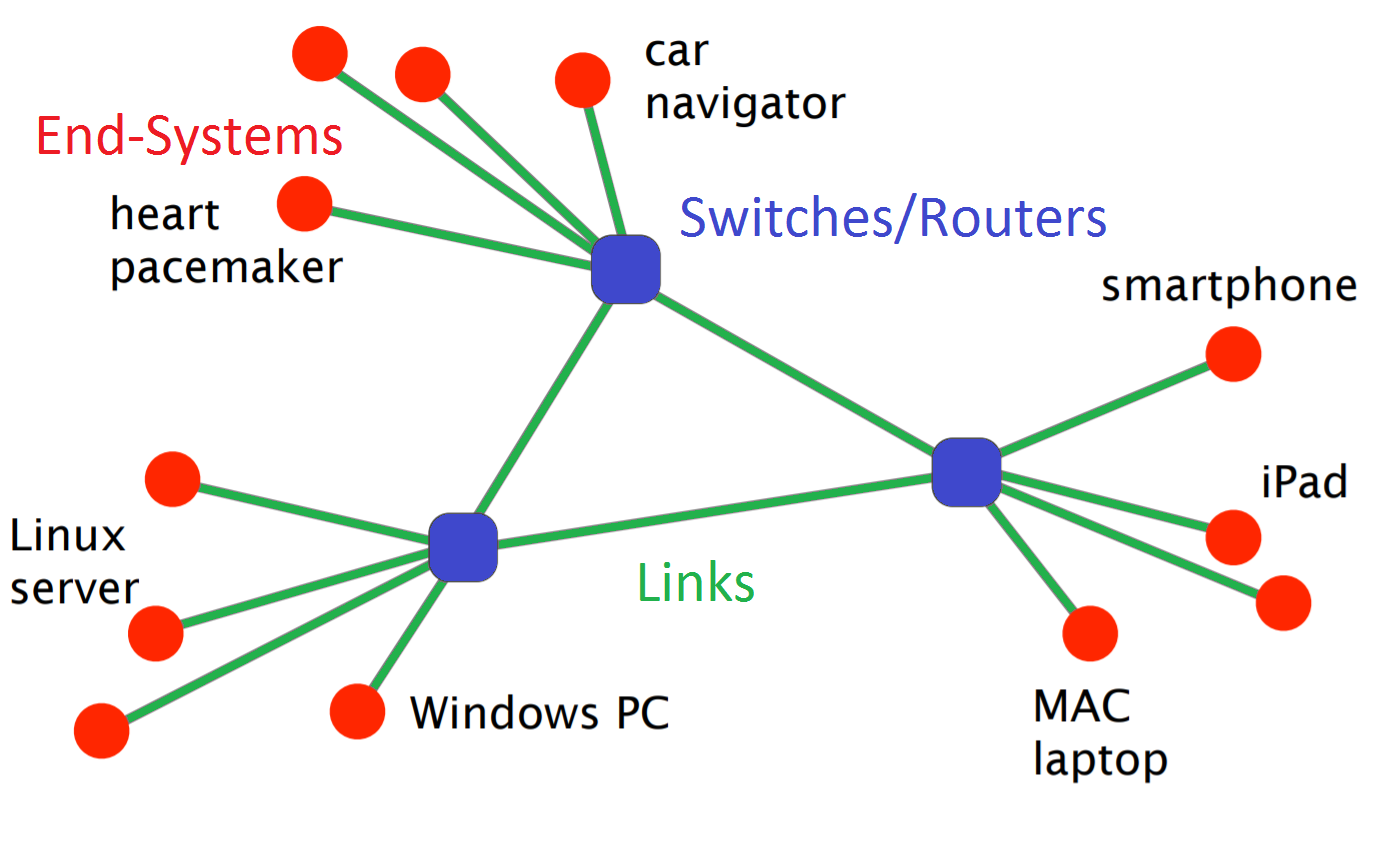
\includegraphics[width= \columnwidth]{images/Overview/network_components.png}
				The internet is a network of networks. The Internet Service Providers (ISP) provide internet to their customers.\\
				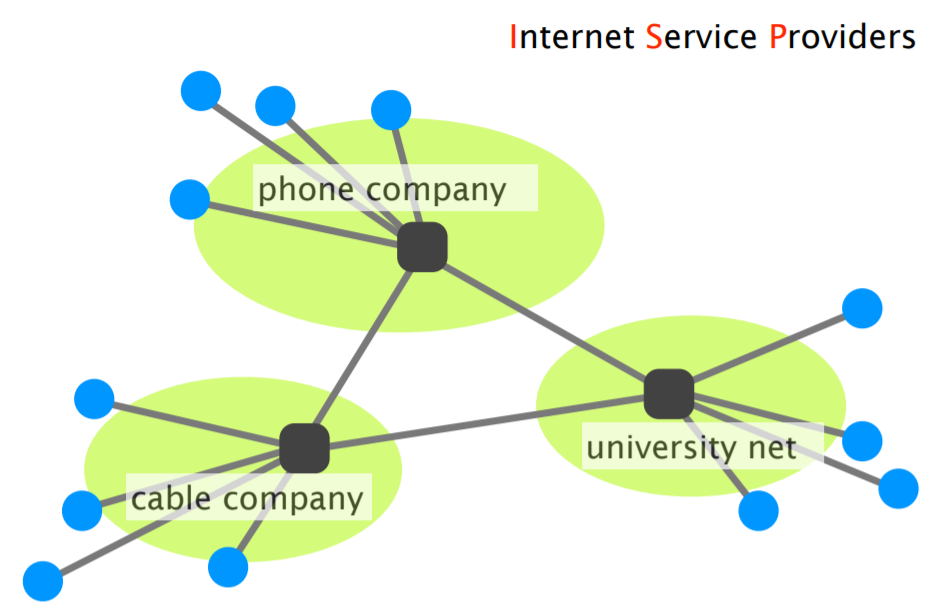
\includegraphics[width= \columnwidth]{images/Overview/ISP.png}
				\columnbreak
			
				There exists a huge amount of \textbf{access technologies: }
				\begin{itemize}[noitemsep]
					\item \textbf{Ethernet} $\vert$ most common, symmetric (Up- and Down-stream same bandwidth)
					\item \textbf{DSL} $\vert$ phone lines, asymmetric (Up- and Down-stream NOT same bandwidth)
					\item \textbf{CATV} $\vert$ via cable TV, shared
					\item \textbf{Cellular} $\vert$ Smart phones 
					\item \textbf{Satellite} $\vert$ remote areas
					\item \textbf{FTTH} $\vert$ fiber to the home
					\item \textbf{Fibers} $\vert$ Internet backbone 
					\item \textbf{Infiniband} $\vert$ High performance computing 
				\end{itemize}
			\subsection{How is it shared?}
				So far we discussed the "last mile" of the Internet.\\
				3 must-have \textbf{requirements} of a good network topology: 
				\begin{itemize}
					\item \textbf{Tolerate failure} $\vert$ several path between src and dst.
					\item \textbf{Sharing to be feasible (praktikabel) \& cost effective } $\vert$ not too much links 
					\item \textbf{Adequate per-node capacity} $\vert$ not to few links 
				\end{itemize}
				The Design of the Internet is a mix of full-mesh, chain and bus which is an optimization of the above requirements. This topology is called a \textbf{switched network}.
				\vspace{-0.5cm}
				%\vspace{-\topsep}
				\begin{itemize}[noitemsep,topsep=0pt]
					\item \textcolor{ForestGreen}{Advantages:}
					\begin{itemize}
						\item \textcolor{ForestGreen}{Sharing and per-node capacity can be adapted to fit the network needs.}
					\end{itemize} 
					\item \textcolor{Red}{Disadvantages:}
					\begin{itemize}
						\item \textcolor{Red}{Require smart devices to perform; forwarding, routing, resource allocation (Zuweisung) }
					\end{itemize} 
				\end{itemize} 
				In a switched network links and switches are shared between flows.
				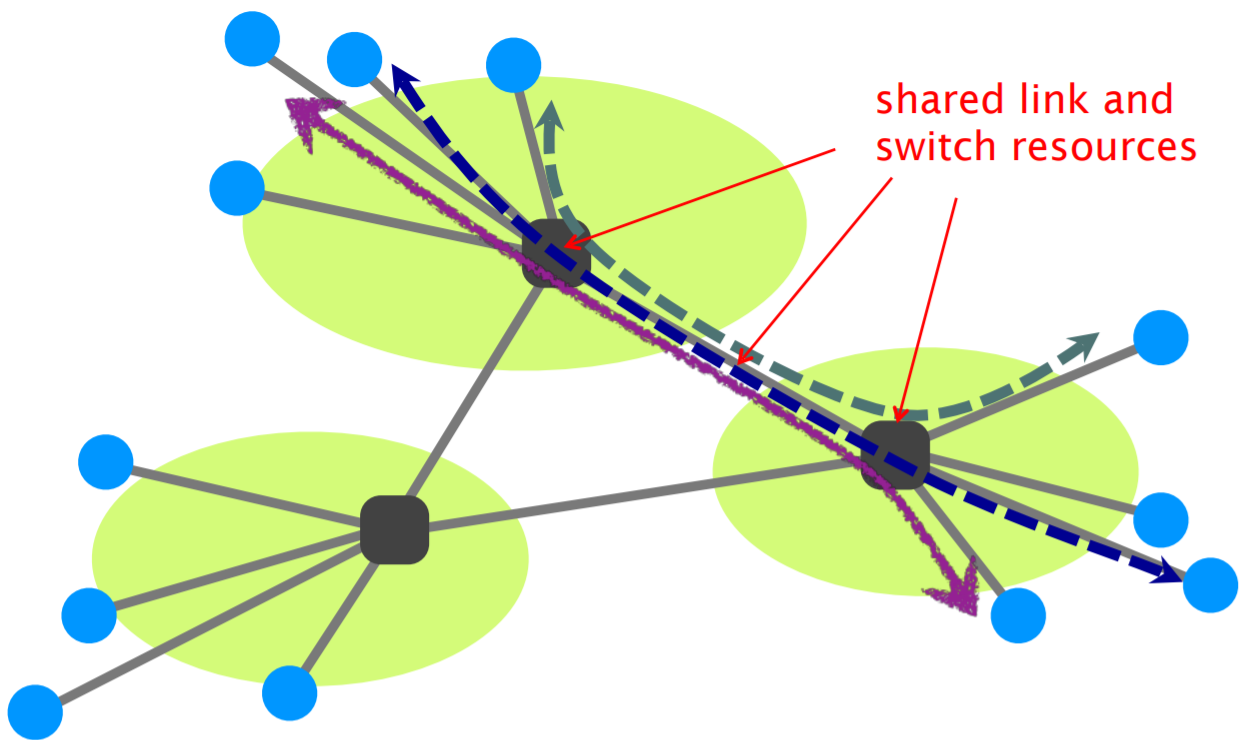
\includegraphics[width= \columnwidth]{images/Overview/link_switch_sharing.png}
				\columnbreak
				
				There exist two approaches of sharing, both are examples of statistical multiplexing: 
				\begin{itemize}
					\item \textcolor{red}{\textbf{Reservation}}\\
						  principle: reserve needed bandwidth in advance\\
						  multiplexing: at the flow-level\\
						  implementation: \textbf{circuit-switching}  
					\item \textcolor{red}{\textbf{On-demand}}\\
						  principle: send data when you need\\
						  multiplexing: at the packet-level\\
						  implementation: \textbf{packet-switching}
				\end{itemize}
				\textbf{Circuit-Switching:}
				\vspace{-0.5cm}
				\begin{itemize}[noitemsep]
					\item Relies on the Resource Reservation Protocol.
					\item The efficiency depends on how utilized the circuit is once established. The circuit can be mostly idle or just be used for a small amount of time (bad).
					\item It doesn't route around trouble 
				\end{itemize}
				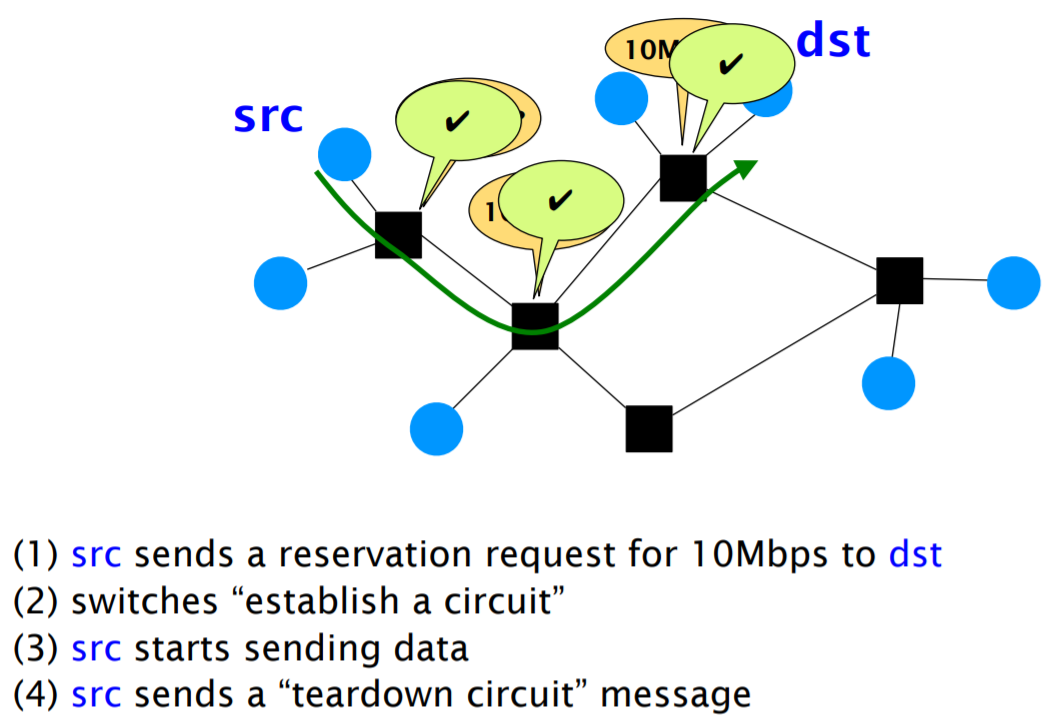
\includegraphics[width=\columnwidth]{images/Overview/circuit_switching.png}
				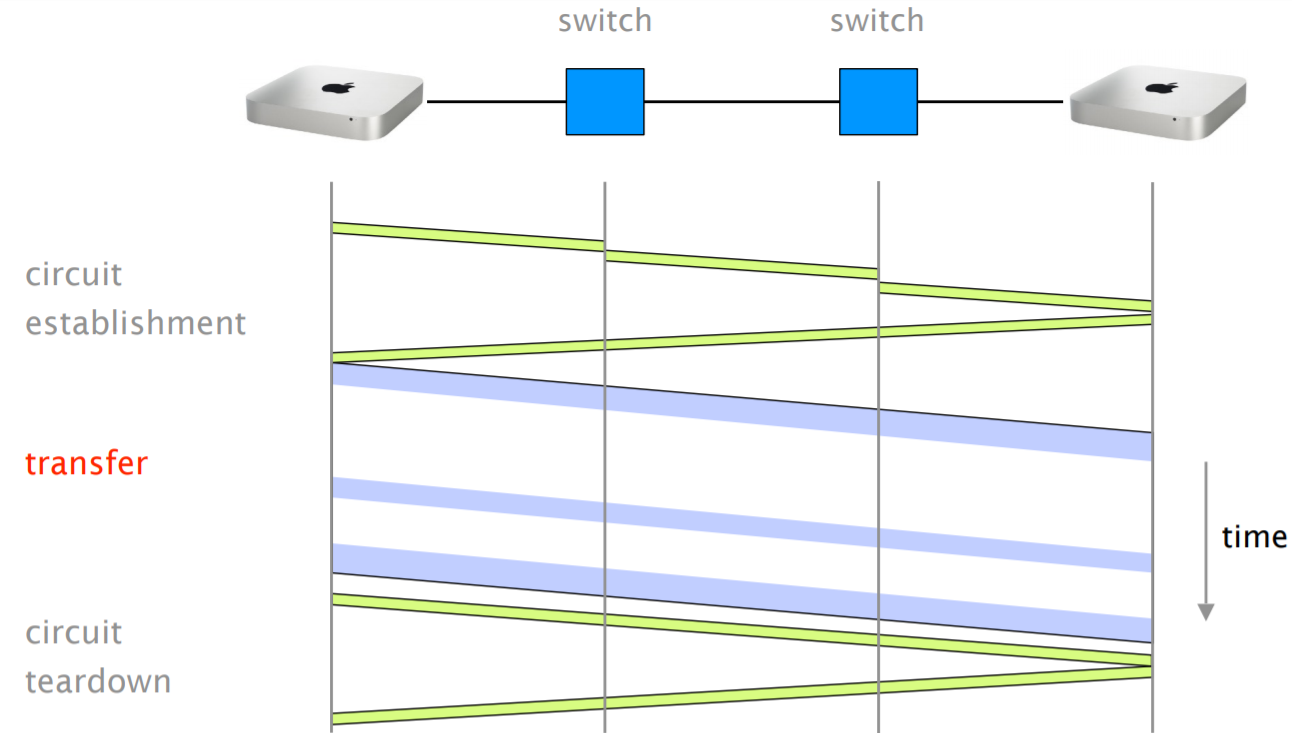
\includegraphics[width=\columnwidth]{images/Overview/circuit_switching_transfer.png}
				\begin{itemize}[noitemsep]
					\item \textcolor{ForestGreen}{Advantages:}
					\begin{itemize}
						\item \textcolor{ForestGreen}{Predictable performance} 
						\item \textcolor{ForestGreen}{Simple \& fast switching (once circuit established)}
					\end{itemize}
					\item \textcolor{red}{Disadvantages:}
					\begin{itemize}
						\item \textcolor{red}{Inefficient if traffic is bursty or short}
						\item \textcolor{red}{Complex circuit setup/teardown (adds delay to transfer)}
						\item \textcolor{red}{Requires new circuit upon failure}
					\end{itemize} 
				\end{itemize}
				\columnbreak
				
				\textbf{Packet-Switching:}
				\vspace{-0.2cm}
				\begin{itemize}[noitemsep]
					\item Data transfer is done using independent packets 
					\item Since packets are not coordinated, they can clash with each other \
					\item To absorb transient overload, packet switching relies on buffers 
					\item It routes around trouble on the fly
				\end{itemize}
				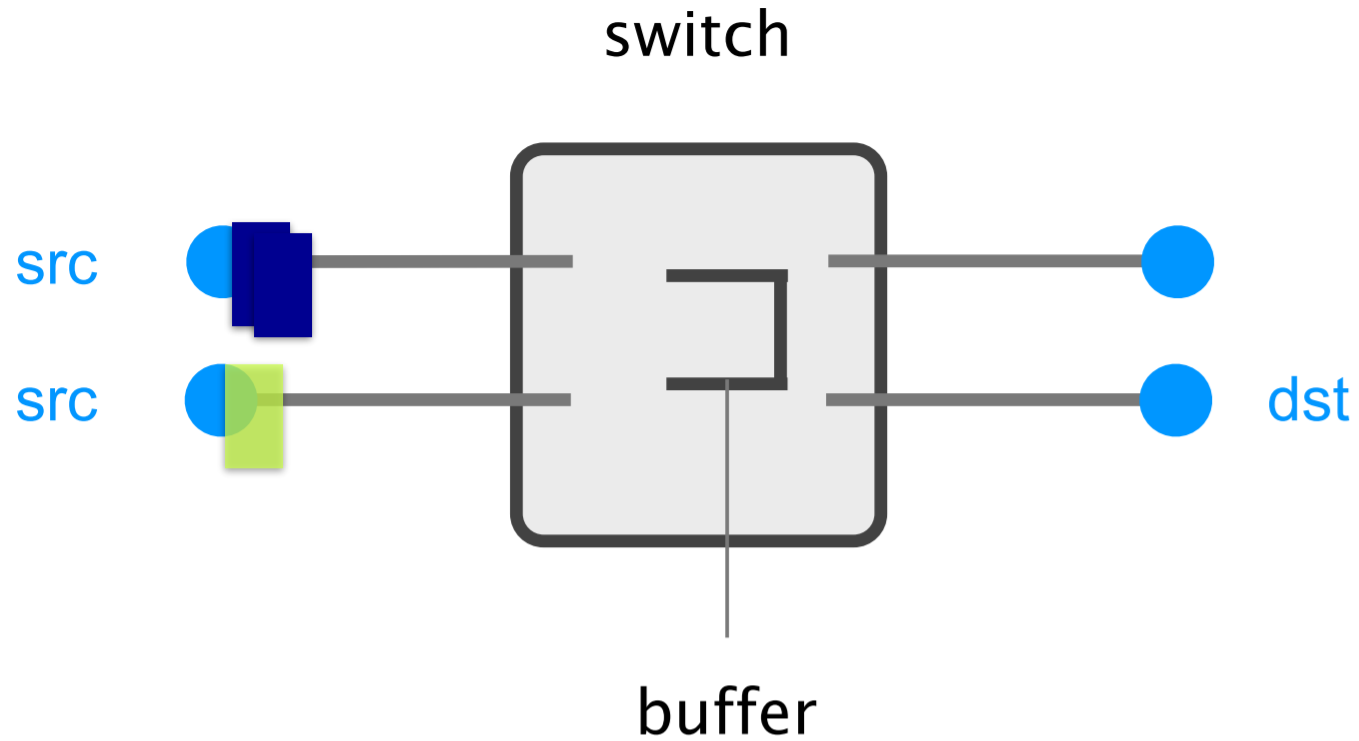
\includegraphics[width=\columnwidth]{images/Overview/packet_switching_buffer.png}
				\begin{itemize}[noitemsep]
					\item \textcolor{ForestGreen}{Advantages:}
					\begin{itemize}
						\item \textcolor{ForestGreen}{Efficient use of resources} 
						\item \textcolor{ForestGreen}{Simpler to implement}
						\item \textcolor{ForestGreen}{Route around trouble}
					\end{itemize}
					\item \textcolor{red}{Disadvantages:}
					\begin{itemize}
						\item \textcolor{red}{unpredictable performance}
						\item \textcolor{red}{Requires buffer management and congestion (Stau) Control}
					\end{itemize} 
				\end{itemize}
				Packet-switching beats circuit-switching with respect to \textbf{resiliency} (robustness) and \textbf{efficiency}. 
				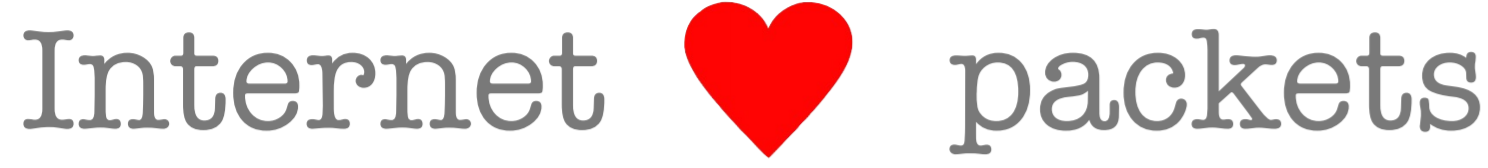
\includegraphics[width=\columnwidth]{images/Overview/internet_loves_packets.png}
			\newpage
			
			\subsection{How is it organized?}
				The Internet has a hierarchical structure and consists of about 60'000 networks: 
				\begin{itemize}[noitemsep]
					\item \textbf{Tier-1} (international)
					\begin{itemize}
						\item have no provider 
						\item $\approx$12 networks
					\end{itemize}
					\item \textbf{Tier-2} (national)
					\begin{itemize}
						\item provide transit to Tier-3s
						\item have at least one provider 
						\item $\approx$1'000s networks 	
					\end{itemize}
					\item \textbf{Tier-3} (local)
					\begin{itemize}
						\item do not provide any transit
						\item have at least one provider
						\item 85-90\% 
					\end{itemize}
				\end{itemize}
				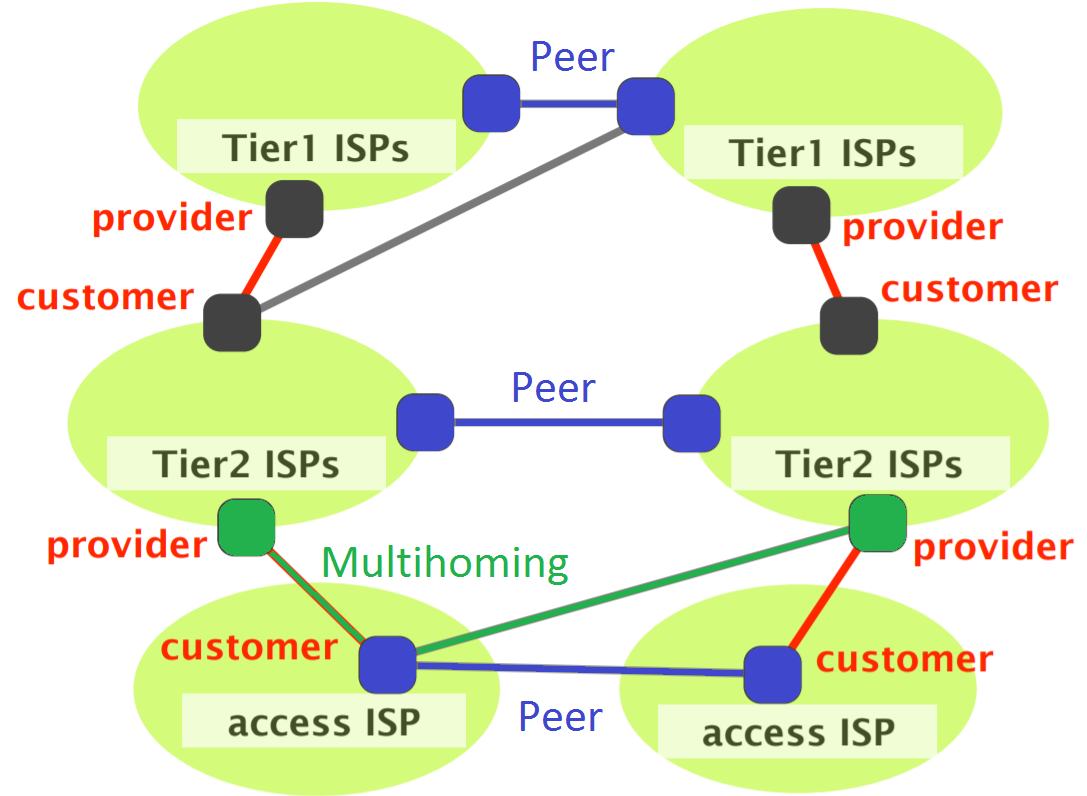
\includegraphics[width=\columnwidth]{images/Overview/hirarchy.png}
				Some networks have an incentive (Anreiz) to connect directly, to reduce their bill with their own provider (direct traffic flow between them). This is known as \textcolor{Blue}{\textbf{peering}}\par
				
				\textbf{IXPs} (Internet Exchange Points): provide Internet connection for Tier2 and other providers. Only have \textcolor{Blue}{\textbf{peering-connections}} . 
				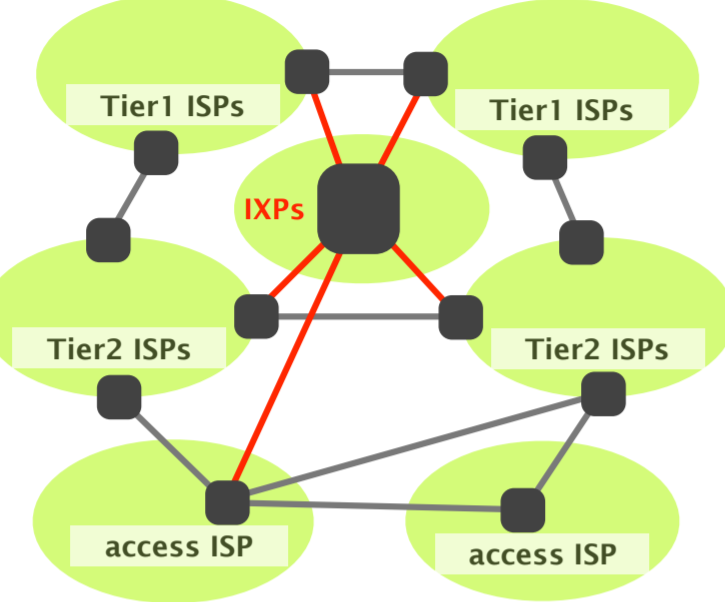
\includegraphics[width=\columnwidth]{images/Overview/IXPs.png}
				\subsection{How does communication happen?}
				Use \textbf{protocols} to enable communication between processes in different networks. Protocols are like a conversation convention. There are thousands of different protocols. Subdivide in different \textbf{layers} to keep stuff simple (Modularity).
				\begin{center}
					\textbf{5 Layer Model}\\
					\Rotatebox{270}{
						\begin{tabular}{l l l l l}
							  & Layer & service provided & role & protocol \\
							\hline						
							L5& Application  & network access & exchanges \textbf{messages} btw. proc. & HTTP, SMTP, FTP, SIP, ...  \\ 
							\hline 
							L4& Transport & end-to-end delivery & transport \textbf{segments} btw. end-sys.&TCP, UDP, SCTP \\ 
							\hline 
							L3& Network  & global best-effort delivery& move \textbf{packets} around the network&IP \\ 
							\hline 
							L2& Link & local best effort delivery& move \textbf{frames} across a link& Ethernet, Wifi, DSL, LTE,... \\ 
							\hline 
							L1& Physical & physical transfer bits & move \textbf{bits} across medium & copper, fiber, coax, ...\\ 
						\end{tabular}
					}
				\end{center}
				\par 
				Each layer provides a service to the layer above by using the layer below. Physical is foundation and everything is then built on top. 
				%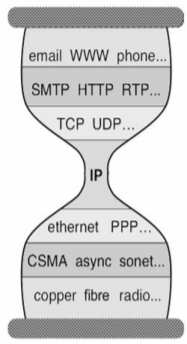
\includegraphics[width=\columnwidth]{images/Overview/clock.png}
				Each layer has a \textbf{unit of data} and is implemented with different protocols and technologies (HW/SW). We can see shift to more HW because of speed. 
				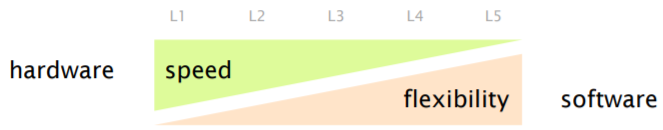
\includegraphics[width=\columnwidth]{images/Overview/hw_sw.png}
				Each layer takes message from above and encapsulates with its own \textbf{header} and/or \textbf{trailer}. 
				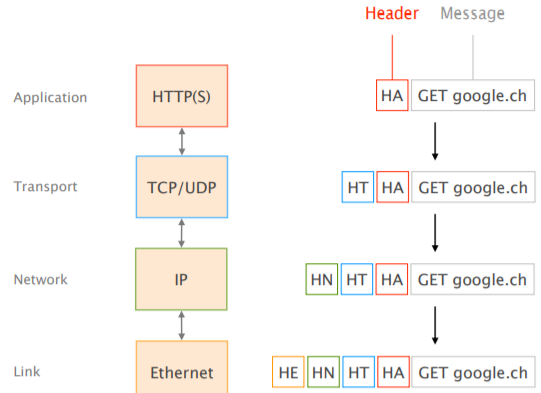
\includegraphics[width=\columnwidth]{images/Overview/header_adding.png}
				\begin{itemize}[noitemsep]
					\item \textbf{Switches} act as a \textbf{L2 gateway}
					\item \textbf{Routers} act as a \textbf{L3 gateway}
				\end{itemize}
			
				\subsection{How do we characterize the network?}
				We characterize the network with:
				\begin{itemize}[noitemsep]
					\item \textbf{Delay}	
					\item \textbf{Loss}
					\item \textbf{Throughput} 
				\end{itemize}
				\textbf{Delay}
				\vspace{-0.2cm}
				\begin{itemize}[noitemsep]
					\item[$\rightarrow$] transmission $\vert$ link property
					\item[$\rightarrow$] propagation $\vert$ link property
					\item[$\rightarrow$] processing $\vert$ traffic $\vert$ mostly tiny
					\item[$\rightarrow$] queuing $\vert$ traffic $\vert$ hardest to evaluate
					\begin{itemize}
						\item[$-$] arrival rate at the queue
						\item[$-$] transmission rate of outgoing link
						\item[$-$] traffic burstiness 
					\end{itemize}
					$\text{traffic intensity} = \dfrac{L\cdot a}{R}$\\
					$a = \text{average packet arrival rate [packet/sec]} $\\
					$R = \text{transmission rate of outgoing link [bit/sec]} $\\
					$L = \text{fixed packet length [bit]} $	
				\end{itemize}
			\textbf{Loss}\\
			If the buffer of a queue is full, it drops packets and hence the packets are lost.\par
			\textbf{Throughput}\\
			To compute throughput one has to consider the bottleneck link
			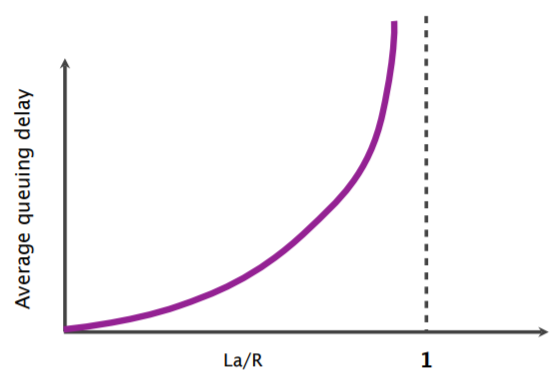
\includegraphics[width=\columnwidth]{images/Overview/traffic_intensity.png}
			As technology improves , throughput increases \& delays are getting lower, except for propagation $\rightarrow$ content delivery networks move content closer to you (e.g. akamai).
			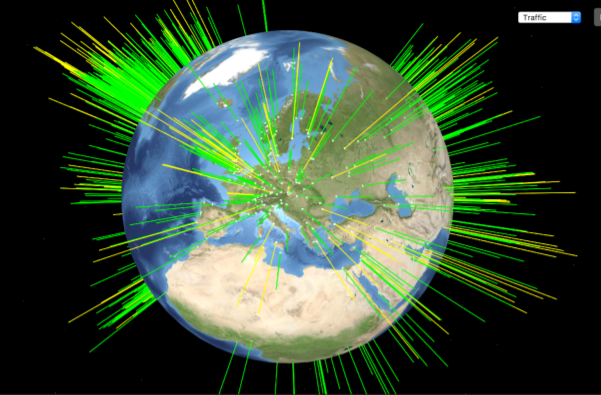
\includegraphics[width=\columnwidth]{images/Overview/akamai.png}
			\newpage 
			
			\section{Concepts}
			\subsection{Routing}
			How do you guide \textbf{IP packet}s from a source to a destination? \\
			Like an envelope, packets have a \textcolor{LimeGreen}{\textbf{header}} and a \textcolor{Orange}{\textbf{payload}}.\\ 
			\begin{center}
			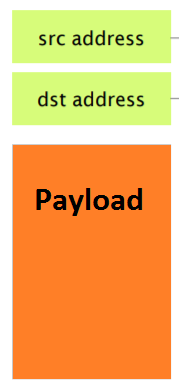
\includegraphics[height=0.4\columnwidth]{images/Concepts/IP_packet.png}
			\end{center}
			Routers forward IP packets \textbf{hop-by-hop}. Routing is mostly not symmetrical (to/back not the same). Routers locally look up their \textbf{forwarding table} to know where to send the packet. Forwarding decisions necessarily depend on the \textbf{destination}, but also can depend on others (source, input port).\\
			In addition to data-plane routers also have a control plane consisting of:
			\vspace{-0.2cm}
			\begin{itemize}[noitemsep]
				\item Routing
				\item Configuration
				\item Statistics
				\item ... 
			\end{itemize}  
			\textbf{Routing} is the control-plane process that \textbf{computes} and \textbf{populates} the forwarding tables.
			\begin{center}
				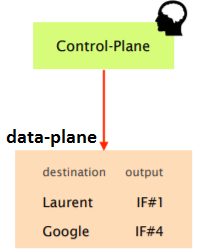
\includegraphics[height=0.4\columnwidth]{images/Concepts/control_data_plane.png}
			\end{center}
			\textbf{Forwarding vs. Routing}\\
			\vspace{0.1cm}	
			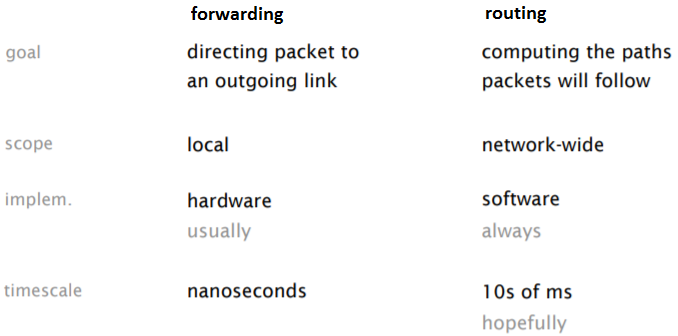
\includegraphics[width=\columnwidth]{images/Concepts/forwarding_vs_routing.png}
			A global forwarding state is valid if and only if:
			\begin{itemize}[noitemsep]
				\item No dead ends
				\item No loops
			\end{itemize} 
		
			\subsubsection{Verifying that a forwarding state is valid}
			It's easy to verify that a routing state is valid. \\
			Simple algorithm: 
			\vspace{-0.1cm}
			\begin{enumerate}[noitemsep]
				\item Mark all outgoing ports with an arrow
				\item Eliminate all link with no arrow 
				\item Sate is valid iff the remaining graph is a \textbf{spanning-tree}
			\end{enumerate} 
			See the following pictures for an example with a resulting spanning tree and one with no spanning tree, hence no valid forwarding state.
			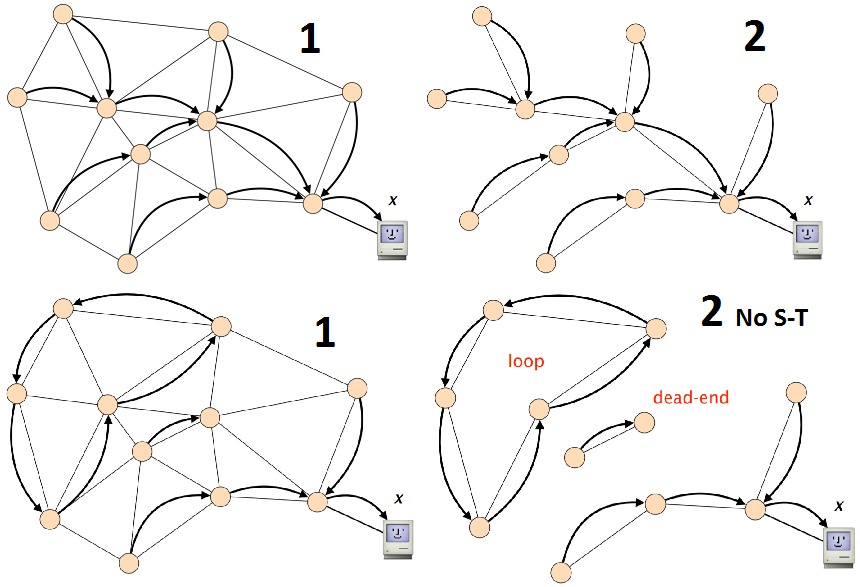
\includegraphics[width=\columnwidth]{images/Concepts/check_s_t.png}
			 
			\subsubsection{How to compute forwarding states}
			Producing valid routing state is harder $\rightarrow$ prevent dead ends (easy) \& loops (hard). Prevent loops is the hard part, this is where routing protocols differ. There are three ways to compute valid routing state: 
			\begin{enumerate}[noitemsep]
				\item Use tree-like topologies $\vert$ Spanning-tree
			 	\item Rely on a global network view $\vert$ Link-state
			 	\item Rely on distributed computation $\vert$ Distance vector 
		 	\end{enumerate}
			In the Internet we use 3., because it is not possible to make precise map of whole Internet.\\
			In Networks we use 2.\\
			Inside (part of) Networks we use 1. \par
			
			\textbf{1. Tree-like topologies}\\
			The easiest way to avoid loops is to route traffic in a loop free topology (Sherlock). Simple algorithm: 
			%\vspace{-0.2cm}
			\begin{enumerate}[noitemsep]
				\item Take an arbitrary topology
				\item Build a spanning tree and ignore all other links
				\item Done!
			\end{enumerate}
			It works, because spanning trees only have one path between any two nodes. There are numerous tress for a topology and they vary in efficiency. \\
			Once we have an spanning tree, forwarding is easy $\rightarrow$ just \textbf{flood} the packets everywhere (see picture below). This is very \textbf{inefficient}. 
			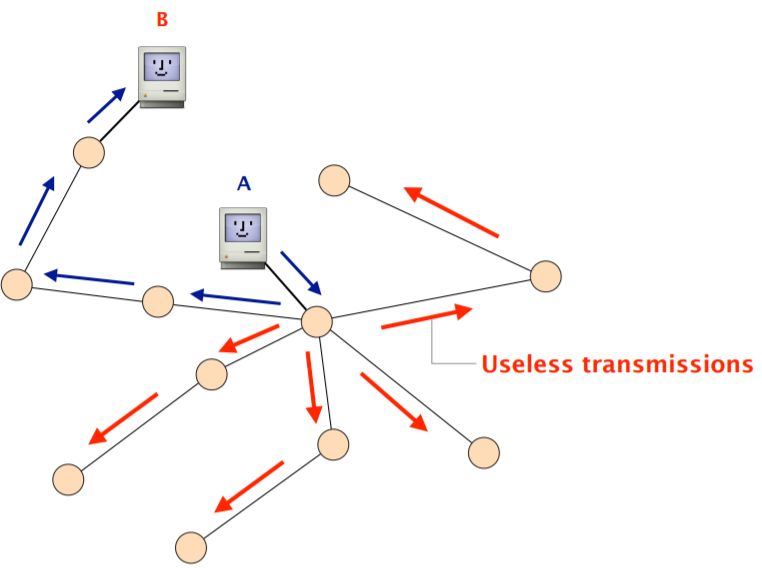
\includegraphics[width=\columnwidth]{images/Concepts/flooding_1.png}
			Solution: Nodes can \textbf{learn} how to reach nodes by remembering where packets came from. Ethernet works just like that. Learning is \textbf{topology-dependent!}\\
			Routing by flooding on a spanning tree (in a nutshell):
			\begin{itemize}[noitemsep]
				\item Flood first packet to node you're trying to reach\\ $\rightarrow$ all switches learn where you are
				\item When destination answers, some switches learn where it is\\
				$\rightarrow$ some because packet to you is not flooded anymore
				\item The decision to flood or not is done on each switch\\ $\rightarrow$ depending on who has communicated before 
			\end{itemize}
			\begin{itemize}[noitemsep]
				\item \textcolor{ForestGreen}{Advantages:}
				\begin{itemize}
					\item \textcolor{ForestGreen}{Plug-and-Play (no config. needed)} 
					\item \textcolor{ForestGreen}{Automatically adapts to moving host}
				\end{itemize}
				\item \textcolor{red}{Disadvantages:}
				\begin{itemize}
					\item \textcolor{red}{Mandate a spanning tree (eliminate many links form the topology)}
					\item \textcolor{red}{Slow to react to failures / host movements}
				\end{itemize} 
			\end{itemize}
			
			\textbf{2. Rely on a global network view}\\
			If \textbf{each routers} knows the entire graph, it can \textbf{locally} compute paths to all other nodes. Once a node \textit{u} knows the entire topology, it can compute shortest paths using \textbf{Dijkstra's algorithm}:
			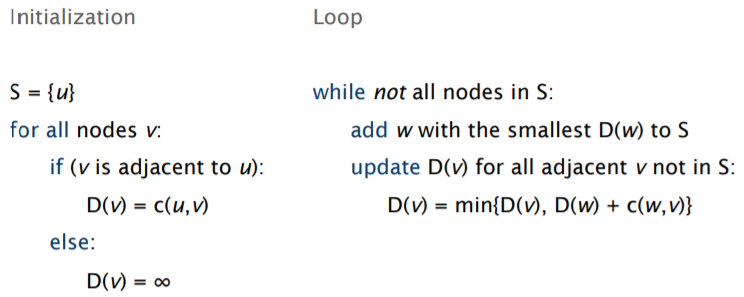
\includegraphics[width=\columnwidth]{images/Concepts/Dijkstra.png}
			$u$ is the node running the algorithm\\
			$c(u,v)$ is the weight of the link connecting $u$ and $v$. \\
			$D(v)$ is the smallest distance currently known by $u$ to reach $v$.\\
			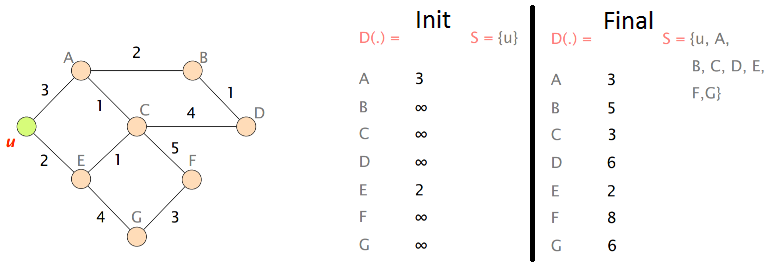
\includegraphics[width=\columnwidth]{images/Concepts/Dijkstra_example.png} 
			Normally the algorithm has $\mathcal{O}(n^2)$ complexity ($n$ being the number of nodes), but with the help of a heap (data-structure...) the complexity can be brought down to $\mathcal{O}(n\log n)$, which is really \textbf{efficient}.\\
			From the shortest paths, $u$ can directly compute its forwarding table! 
		    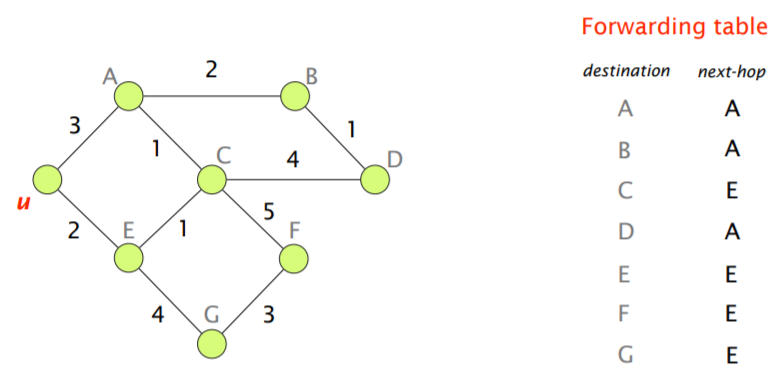
\includegraphics[width=\columnwidth]{images/Concepts/forwarding_table.png} 	 
		    \textbf{How do we know cost?}\\
		   	Initally, routers only knwo their ID and their neighbors and the cost to reach them. They then build message known as Link-state (with neighbors and their cost/weight) and flood it in the network\\
		    $\rightarrow$ At the end of the flooding process everyone should have the exact same view of the network. \\
		    I can configure wight of links \textbf{static} by hand (Dijkstra will converge), or \textbf{dynamic} (may be problematic).\par 
		    
		    \textbf{3. Rely on distributed computation}\\
		    Paths can be computed in distributed computation.\\
		    Let $d_x(y)$ be the cost of the least-cost path known by $x$ to reach $y$. \\
		    Each node bundles these distances into one message (vector) that it \textbf{repeatedly} sends to all its neighbors. \\
		    Each node updates its distances based on neighbors vectors:\\
		    $d_x(y)=\min\{c(x,v)+d_v(y)\}$, overall neighbors $v$.\\
		    This leads to a recursive computation of the shortest path, the result must be the same as Dijkstra algorithm! 
		    Example: Compute shortest path from $u$ to D:\\
		    $d_u(D)=\min\{c(u,A)+d_A(D), c(u,E)+d_E(D)\}$\\
		    $\downarrow$\\
		    $d_A(D)=\min\{c(A,B)+d_B(D), c(A,C)+d_C(D)\}=\min\{2+1,1+4\}=3$\\
		    $\downarrow$\\
		    $d_E(D)=\min\{c(E,C)+d_C(D), c(E,G)+d_G(D),c(E,u)+d_u(D)\}=5$\\
		    $\downarrow$\\
		    $d_u(D)=\min\{3+d_A(D), 2+d_E(D)\}=6$\\
		    As before $u$ can directyl infer its forwarding table, by directing the traffic to its best neighbor (the one which advertises the smallest cost). Evaluating the complexity of DV is harder. 
		    
		    \subsection{Reliable delivery}
		    How do you ensure reliable transport on top of best-effort delivery?\\
		    \textbf{Goals:}
		    \begin{itemize}[noitemsep]
		    	\item Keep the network simple,dumb\\
		    	$\rightarrow$ make it easy to build/operate network
		    	\item Keep application as network unaware as possible\\
		    	$\rightarrow$ Developer should focus on app, not network 
		    \end{itemize}
	    	\textbf{Design:}
	    	\begin{itemize}
	    		\item Implement reliability in-between, in the networking stack\\
	    		$\rightarrow$ relive the burden from both the app and network
	    	\end{itemize}
    		The Internet puts \textbf{reliability in L4}, just above the network layer.\\
    		What can the mean Internet do to our IP-packets:
    		\begin{itemize}[noitemsep]
    			\item Lost or delayed
    			\item Corruption
    			\item Reordering
    			\item Duplication 
    		\end{itemize}
    		We have four goals of reliable transfer:
    		\begin{itemize}[noitemsep]
    			\item \textbf{Correctness:} ensure data is delivered, in order, and untouched
    			\item \textbf{Timeliness:} minimize time until data is transferred 
    			\item \textbf{Efficiency:} optimal use of bandwidth
    			\item \textbf{Fairness:} play well with concurrent communications  
    		\end{itemize}
    		\textbf{Correctness:}\\
    		A reliable transport design is correct iff:\\
    		A packet is \textcolor{Red}{always resent} if the previous packet was lost or corrupted. A packet may be resent at other times.\\
    		Note: It is \textcolor{Red}{ok to give} up after a while, but it must be announced to the application.\par
    		
    		Designing a \textcolor{Red}{correct}, \textcolor{Red}{timely}, \textcolor{Red}{efficient} transport mechanism knowing that packets can get \textcolor{Red}{lost} (focus on mentioned aspects):
    		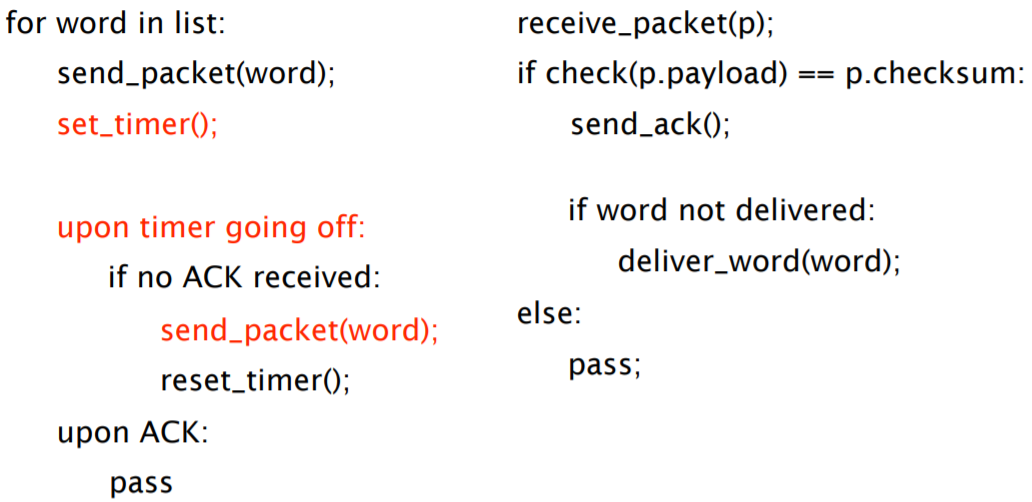
\includegraphics[width=\columnwidth]{images/Concepts/send_packet.png} 	 
    		There is a clear tradeoff between timeliness and efficiency in the selection of the timeout value. Big challenge to choose optimal value.\\
    		Small timers: Risk of \textbf{unnecessary retransmissions}\\
    		Large timers: Risk of \textbf{slow transmission} \par
    		
    		To improve timeliness just send multiple packets at the same time and not wait to ACK every packet. \\
    		Approach: 
    		\begin{itemize}[noitemsep]
    			\item Add sequence number to every packet
    			\item Add buffers to sender and receiver: 
    			\begin{itemize}
    				\item[$-$] Sender: store packets sent \& not acknowledged
    				\item[$-$] Receiver: store out-of-order packets received
    			\end{itemize}
    		\end{itemize} 
    		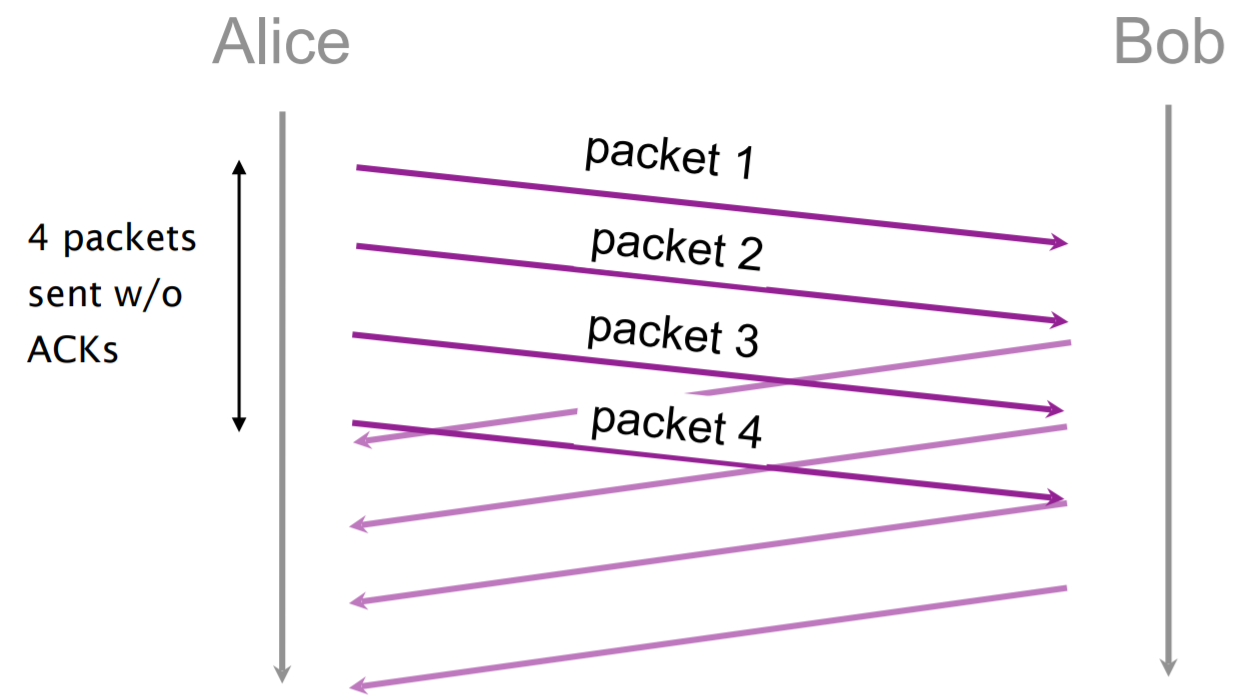
\includegraphics[width=\columnwidth]{images/Concepts/packets_wo_ack.png} 	 
    		One problem that can occur is: 
    		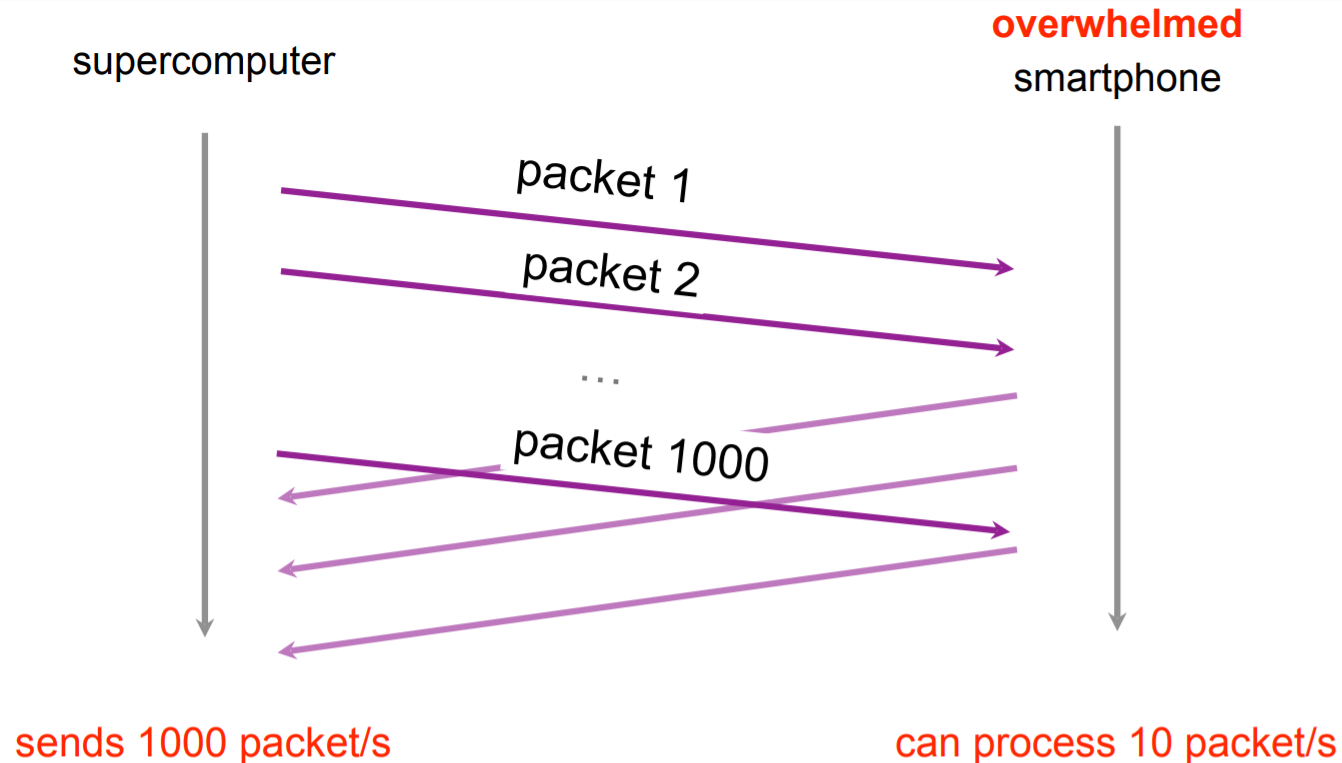
\includegraphics[width=\columnwidth]{images/Concepts/packets_wo_ack_problem.png} 
    		To solve this issue  we need a mechanism for \textcolor{Red}{\textbf{flow control}}.
    		Using a \textbf{sliding window} is one way to do that:
    		\begin{itemize}
    			\item[$-$] Sender keeps a list of the sequence \# it can send.\\
	   			$\rightarrow$ known as the \textit{sending window}
	   			\columnbreak
	   			\item[$-$] Receiver keeps a list of acceptable sequence \#\\
	   			$\rightarrow$ known as the \textit{receiving window }
	   			\item[$-$] Sender and receiver negotiate the window size\\
	   			$\rightarrow$ sending window $\le$ receiving window
    		\end{itemize} 
    		Example with a window-size of 4 packets:
    		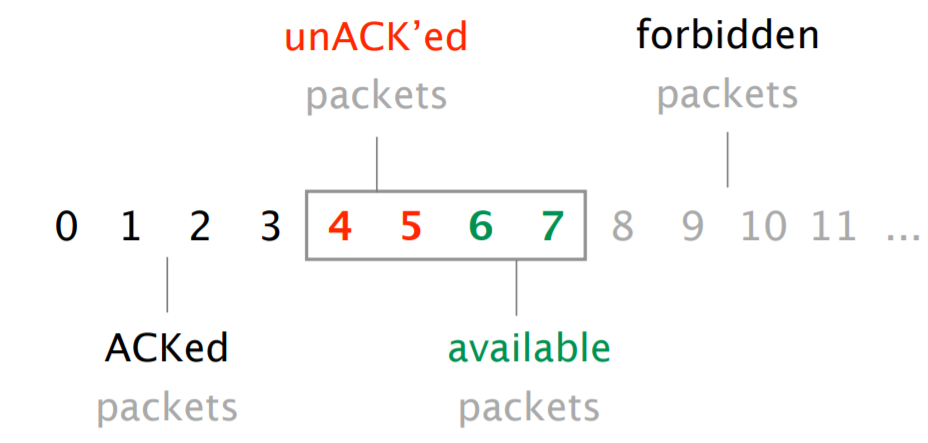
\includegraphics[width=\columnwidth]{images/Concepts/windowsize4_1.png} 
    		%\vspace{0.2cm}
    		Window after sender receives \textcolor{Red}{ACK 4 }
    		%\vspace{0.1cm}
    		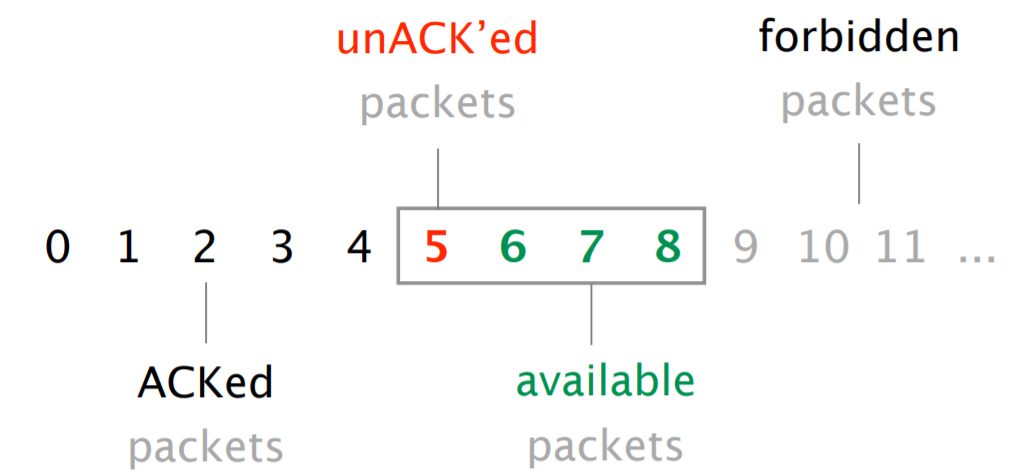
\includegraphics[width=\columnwidth]{images/Concepts/windowsize4_2.png} 
    		Timeliness of the window protocol depends on the size of the sending window.\par
    		
    		\textbf{ACKing individual packets}
    		\vspace{-0.2cm}
    		\begin{itemize}[noitemsep]
    			\item \textcolor{ForestGreen}{Advantages:}
    			\begin{itemize}
    				\item \textcolor{ForestGreen}{Know fate of each packet} 
    				\item \textcolor{ForestGreen}{Simple window algorithm}
    				\item \textcolor{ForestGreen}{Not sensitive to reordering}
    			\end{itemize}
    			\item \textcolor{red}{Disadvantages:}
    			\begin{itemize}
    				\item \textcolor{red}{Unnecessary retransmission upon losses}
    			\end{itemize} 
			\end{itemize}
		
    		\textbf{Cumulative ACKs}\\
   			ACK the highest sequence number for which all the previous packets have been received.
   			\vspace{-0.2cm}
   			\begin{itemize}[noitemsep]
   				\item \textcolor{ForestGreen}{Advantages:}
   				\begin{itemize}
   					\item \textcolor{ForestGreen}{Recover from lost ACKs}
   				\end{itemize}
   				\item \textcolor{red}{Disadvantages:}
   				\begin{itemize}
   					\item \textcolor{red}{Causes unnecessary retransmissions}
   					\item \textcolor{red}{Confused by reordering}
   					\item \textcolor{red}{Incomplete information about which packets have arrived}
   				\end{itemize} 
   			\end{itemize}
   		
   			\textbf{Full information feedback}\\
   			List all packets that have been received highest cumulative ACK, plus any additional packets
   			\vspace{-0.2cm}
   			\begin{itemize}[noitemsep]
   				\item \textcolor{ForestGreen}{Advantages:}
   				\begin{itemize}
   					\item \textcolor{ForestGreen}{Complete information}
   					\item \textcolor{ForestGreen}{Resilient (belastbar) form of individual ACKs}
   				\end{itemize}
   				\item \textcolor{red}{Disadvantages:}
   				\begin{itemize}
   					\item \textcolor{red}{Overhead}
   				\end{itemize} 
   			\end{itemize}
   			
   			With individual ACKs and full information detection of a missing packet is easy (implicit/explicit). \\
   			With cumulative ACKs missing packets are harder to know. \par
   			
   			\textbf{Fairness:}\\
   			Fair is mostly not efficient. Defining what fair is, is not easy. What matters is to \textbf{avoid starvation}. Equal-per-flow is good enough for this. Simply dividing available bandwidth doesn't work.\\
   			We want to give users with small demands what they want and evenly distribute the rest. \textbf{max-min fair allocation} is such that: the lowest demand is maximized $\rightarrow$ the second lowest is maximized $\rightarrow$ the third lowest is maximized and so on...\\
   			\textbf{max-min fair allocation:}
   			\begin{enumerate}[noitemsep]
   				\item Start with all flows at rate 0
   				\item Increase the flows until there is a new bottleneck in the network
   				\item Hold the fixed rate of the flows that are bottlenecked
   				\item Got to step 2 for the remaining flows. 	 
   			\end{enumerate}  
   			Max-min fair allocation can be approximated by increasing window until a loss is detected. \par
   			
   			\textbf{Corruption:}\\
   			Dealing with corruption is easy: Rely on a checksum and treat corrupted packets as lost ones. \par 
   			
   			\textbf{Reordering:}\\
   			Effect depends on ACKing mechanism which is used:\\
   			$\bullet$ Individal ACK: \textcolor{ForestGreen}{no problem}\\
   			$\bullet$ Full feedback: \textcolor{ForestGreen}{no problem}\\
   			$\bullet$ Cumm. ACKs: \textcolor{Red}{Create duplicate ACKs}.\par
   			
   			\textbf{Duplicates:}\\
   			Can lead to duplicated ACKs whose effect depends on the ACKing mechanism: \\
   			$\bullet$ Individual ACK: \textcolor{ForestGreen}{no problem}\\
   			$\bullet$ Full feedback: \textcolor{ForestGreen}{no problem}\\
   			$\bullet$ Cumm. ACKs: \textcolor{Red}{problematic}\par
   			
   			\textbf{Delay:}\\
   			Can create useless timeouts for all designs. It is hard to deal with the different delays which occur over the whole network. How do I set the right amount of timeout?\\
   			\newpage
   			
   			\section{The Link Layer}
   			\subsection{What is a link?}
   			\textbf{Link =  Medium + Adapter}\\
   			Network adapters communicate together through the medium.\\
   			In the link layer we talk about \textbf{Frames} which are sent form one adapter to the other.\\
   			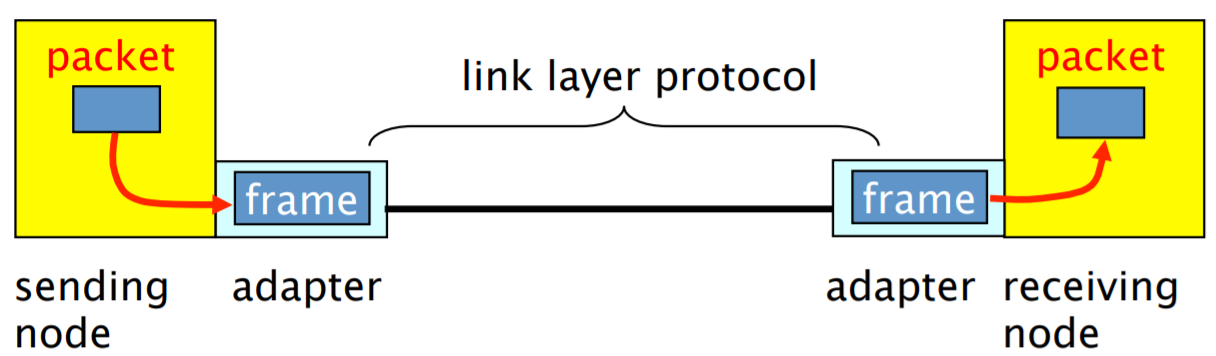
\includegraphics[width=\columnwidth]{images/Link_Layer/link.png} 
   			\textbf{Sender}
   			\vspace{-0.3cm}
   			\begin{itemize}[noitemsep]
   				\item Encapsulate packets in a frame
   				\item add error checking bits, flow control,...
   			\end{itemize}
   			\textbf{Receiver:}
   			\vspace{-0.3cm}
   			\begin{itemize}[noitemsep]
   				\item Look for errors, flow control,...
   				\item Extract packet and passes it to network layer 
   			\end{itemize}
   			Link-Layer provides a best effort delivery service to the network layer, composed od \textbf{5} sub services.
   			\begin{itemize}[noitemsep]
   				\item \textbf{Encoding} $\vert$ represents the 0's and 1's
   				\item \textbf{Framing} $\vert$ encapsulates packet into a frame (header/trailer)
   				\item \textbf{Error detection} $\vert$ detects errors with checksum
   				\item \textbf{error correction} $\vert$ optionally correct errors
   				\item \textbf{Flow Control} $\vert$ pace sending and receiving node 
   			\end{itemize} 
   			
   			\subsection{How do we identify link adapters?}
   			\textbf{M}edium \textbf{A}ccess \textbf{C}ontrol address:
   			\vspace{-0.2cm}
   			\begin{itemize}[noitemsep]
   				\item \textbf{Identify the sender \& receiver adapters} $\vert$ used within a link
   				\item \textbf{Are uniquely assigned} $\vert$ hard coded into adapter
   				\item \textbf{Use a flat space of 48 bits} $\vert$ allocated hierarchically 
   			\end{itemize}
   			The \textcolor{Green}{first} 24 bits blocks are assigned to network adapter vendor by IEEE. (1 Vendor may have more than 1 block.)
   			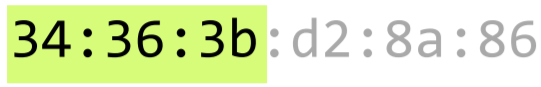
\includegraphics[width=\columnwidth]{images/Link_Layer/first_mac_block.png}
   			The \textcolor{Orange}{second} 24 bits block is assigned by the vendor to each network adapter.(My use the same in geographically different locations!)
   			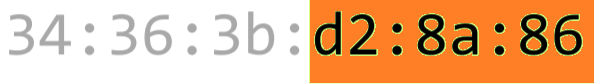
\includegraphics[width=\columnwidth]{images/Link_Layer/second_mac_block.png}
   			broadcast address has set all bits to 1: ff:ff:ff:ff:ff:ff, enables to send a frame to all adapters on the link.\\
   			By default, adapters only decapsulate frames addressed to the local MAC or broadcast address. The promiscuous mode enables to decapsulate everything.\\
   			Why don't we simply use IP-addresses?
   			\begin{enumerate}[noitemsep]
   				\item Links can support any protocol (not just IP) $\vert$ different addresses on different kind of links
   				\item Adapters may move to different locations $\vert$ cannot assign static IP address, it has to change
   				\item \textbf{Adapters must be identified during bootstrap} $\vert$ need to talk to an adapter to give it an IP address 
   			\end{enumerate} 
   			You need to solve two problems when bootstrapping an adapter:
   			\begin{itemize}[noitemsep]
   				\item Who am I? (How do I acquire an IP address $\vert$ MAC-to-IP binding) $\vert$ \textcolor{Red}{Dynamic Host Configuration Protocol DHCP}
   				\item Who are you? (Given an reachable IP-address on a link, how do I find out what MAC to use) $\vert$ IP-to-MAC binding $\vert$ \textcolor{Red}{Address Resolution Protocol ARP}
   			\end{itemize}
   			Network adapters traditionally acquire an IP address using \textbf{DHC}:
   			\begin{enumerate}[noitemsep]
   				\item \textbf{Discovery} $\vert$ Client searching DHCP Server (via broadcast)
   				\item \textbf{Offer} $\vert$ DHCP server sending offer to client
   				\item \textbf{Request} $\vert$ Client request IP from DHCP server
   				\item \textbf{ACK} $\vert$ DHCP server assigns IP and sends ACK 
   			\end{enumerate}
   			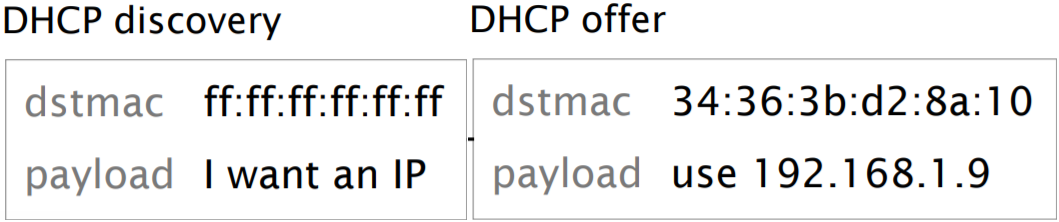
\includegraphics[width=\columnwidth]{images/Link_Layer/DHCP.png}
   			\par 
   			
   			The \textbf{ARP} enables to discover the MAC associated to an IP: 
   			\begin{enumerate}[noitemsep]
   				\item ARP \textbf{Request}: Who has $<$some Ip$>$ tell $<$my IP$>$ to broadcast MAC
   				\item ARP \textbf{Reply}: $<$some IP$>$ is at $<$this MAC$>$
   				\item Requester puts entry in his \textbf{ARP-table}
   			\end{enumerate}
   			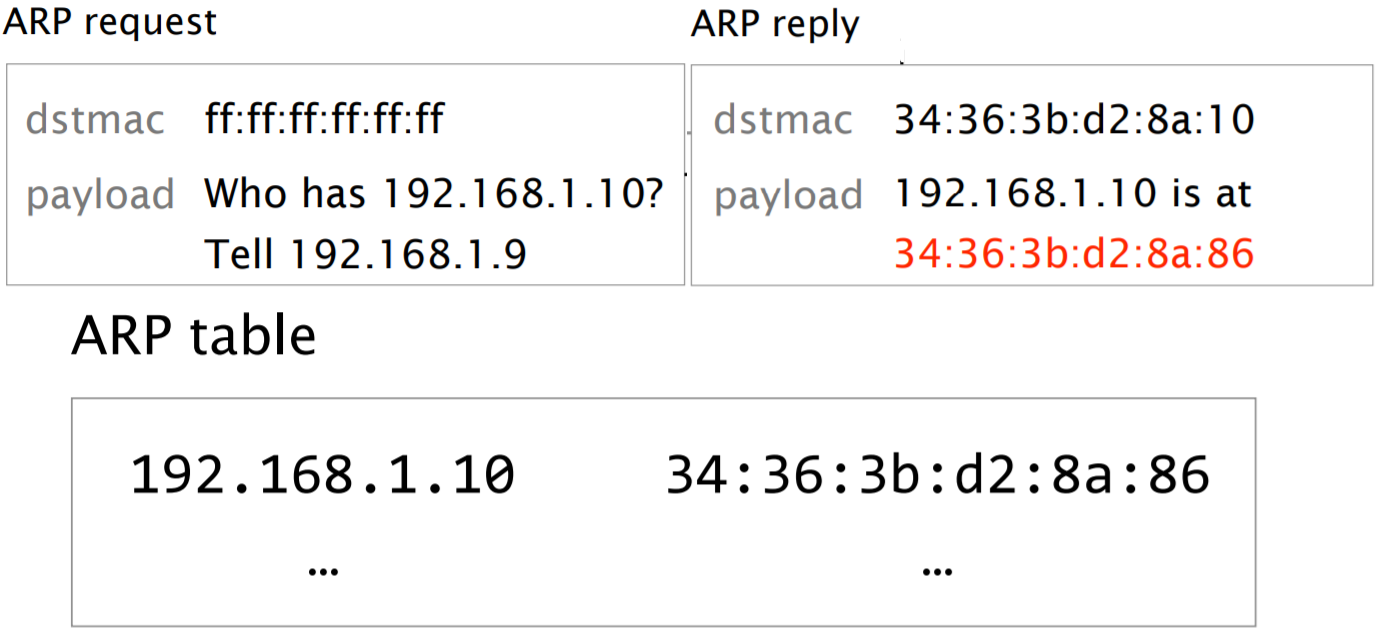
\includegraphics[width=\columnwidth]{images/Link_Layer/ARP.png}
   			
   			\subsection{How do we share a network medium?}
   			Some medium are \textbf{multi-access}: $>1$ host can communicate at same time.\\
   			\textcolor{Red}{Problem: Collision lead to garbled (verstümmelt) data.}\\
   			\textcolor{ForestGreen}{Solution: Distributed algorithm for sharing the channel.}\\
   			Essentially there are three techniques to deal with Multi Access Control (MAC):
   			\begin{itemize}[noitemsep]
   				\item \textbf{Divide the channel into pieces} $\vert$ either in time or frequency
   				\item \textbf{Take turns} $\vert$ pass a token for the right to transmit
   				\item \textbf{Random access} $\vert$ allow collisions, detect them and then recover
   			\end{itemize} 
   			
   			\subsection{What is Ethernet?}
   			\begin{itemize}[noitemsep]
   				\item Was invented as a broadcast technology
   				\item Is the dominant wired LAN technology 
   				\item Has managed to keep up with the speed race
   			\end{itemize}
   			Ethernet offers an \textbf{unreliable} and \textbf{connectionless} service.\\
   			Unreliable:
   			\begin{itemize}[noitemsep]
   				\item[$-$] Receiving adapter does not acknowledge anything
   				\item[$-$] Packets passed to the networks layer can have gaps
   			\end{itemize}
   			Connectionless: 
   			\begin{itemize}[noitemsep]
   				\item[$-$] No handshake between sender and receiver
   			\end{itemize}
   			Traditional Ethernet relies on CSMA/CD (carries-sense multiple access with collision detection). All hosts were on a big bus-cable connected. You needed to sense the cable in order to know if someone is speaking. multiple hosts had access to the medium, while you were speaking you still were listening to detect collisions. CSMA/CD imposes \textbf{limits} to the network length.\\
   			$\mathrm{Network\ length}=\frac{min\ frame\ size\ \cdot\ speed\ of\ light}{2\cdot bandwidth}$\\
   			For this reason Ethernet imposes a minimum packet size of 512 bits.\\
   			Modern Ethernet links interconnect exactly two hosts, in full duplex, rendering collisions impossible. 
   			\begin{itemize}[noitemsep]
   				\item CSMA/CD is only needed for half-duplex communication
   				\item This means the 64 Byte restriction is not strictly needed (but still kept)
   				\item Multiple Access Protocols are still important for wireless communication
   			\end{itemize}
   			The Ethernet header is simple, composed of 6 fields: 
   			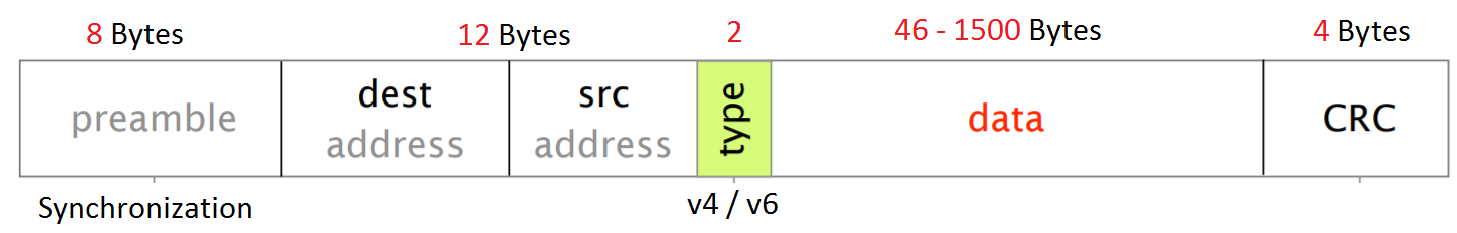
\includegraphics[width=\columnwidth]{images/Link_Layer/eth_header.png}
			Ethernet efficiency is $\approx97.5\%$ (paylod/framesize). 
			
			\subsection{How do we interconnect segments at the link layer?}
			Historically, people connected Ethernet segments together at the physical level with ethernet \textbf{hubs}. Hubs work by repeating bits from one port to all the others (flooding everything). 
			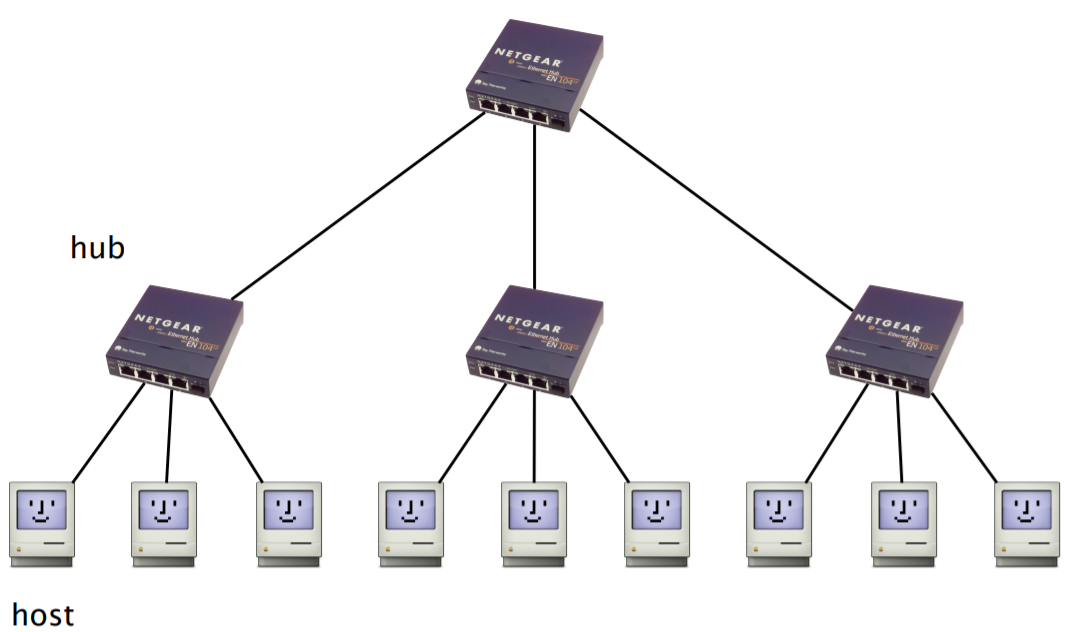
\includegraphics[width=\columnwidth]{images/Link_Layer/hub.png}
			\begin{itemize}[noitemsep]
				\item \textcolor{ForestGreen}{Advantages:}
				\begin{itemize}
					\item \textcolor{ForestGreen}{Cheap, simple}
				\end{itemize}
				\item \textcolor{red}{Disadvantages:}
				\begin{itemize}
					\item \textcolor{red}{Inefficient}
					\item \textcolor{red}{Limited ot one LAN technology}
					\item \textcolor{red}{Limited number of nodes/distances} 
				\end{itemize} 
			\end{itemize}
   			LANs are now almost exclusively composed of Ethernet \textbf{switches}. Switches connect two or more LANs together on the Link layer, actings as L2 gateways. Switches are \textbf{store and forward} devices, they: 
   			\begin{itemize}[noitemsep]
   				\item Extract the DST MAC $\vert$ from the frame
   				\item Look up the MAC in a table $\vert$ using exact match
   				\item Forward the frame $\vert$ on the appropriate port
   			\end{itemize}
   			Similiar to IP routers, except they are one layer below. Switch enables each LAN segment to carry its own traffic (no flooding of network). 
   			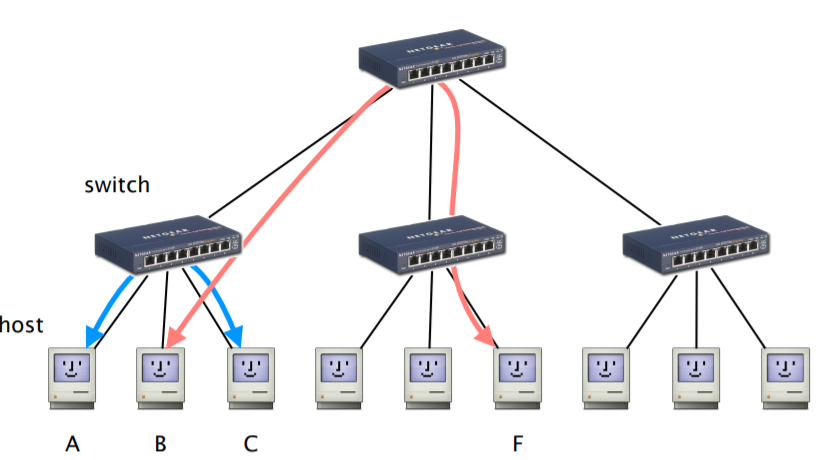
\includegraphics[width=\columnwidth]{images/Link_Layer/switch_network.png}
   			Switches are Plug-and-Play they build their forwarding table on their own.\\
   			The advantages of switches are numerous: 
   			\begin{itemize}[noitemsep]
   				\item \textcolor{ForestGreen}{Advantages:}
   				\begin{itemize}
   					\item \textcolor{ForestGreen}{Only forward frames where needed} $\vert$ avoids unnecessary load on segments
   					\item \textcolor{ForestGreen}{Join segments using different technologies}
   					\item \textcolor{ForestGreen}{Improved privacy} $\vert$ hosts can only snoop traffic traversing their segment
   					\item \textcolor{ForestGreen}{Wider geographic span} $\vert$ separates segments allow longer distance
   				\end{itemize} 
   			\end{itemize}
   			\newpage
   			
   			When Frames arrive:
   			\vspace{-0.2cm} 
   			\begin{itemize}[noitemsep]
   				\item [$-$] Inspect the SRC MAC address
   				\item [$-$] associate the address with the port
   				\item [$-$] Store the mapping in the switch table
   				\item [$-$] Launch a timer to eventually forget the mapping
   			\end{itemize}
   		In case of misses, switches simply flood the network (when in doubt, shout).\\
   		When a frame arrives with an unknown DST $\rightarrow$ forward the frame out all ports, except where the frame arrived from.\\ 
   		Flooding enables \textbf{automatic discovery} of hosts, but with loops the load increases exponentially! Solution: Reduce the network to one logical \textbf{spanning tree}.\\
   		In practice, switches run distributed Spanning-Tree-Protocol (\textbf{STP}). \\
   		Construction of a spanning tree in a nutshell: Switches...
   		\begin{itemize}[noitemsep]
   			\item Elect a root $\vert$ the one with the smallest identifier
   			\item determine if each interface is on the shortest path from the root $\vert$ if not $\rightarrow$ disable it.
   		\end{itemize}
   		For this switches exchange Bridge Protocol Data Unit (BPDU) messages\\
   		Each Switch X iteratively sends: 
   		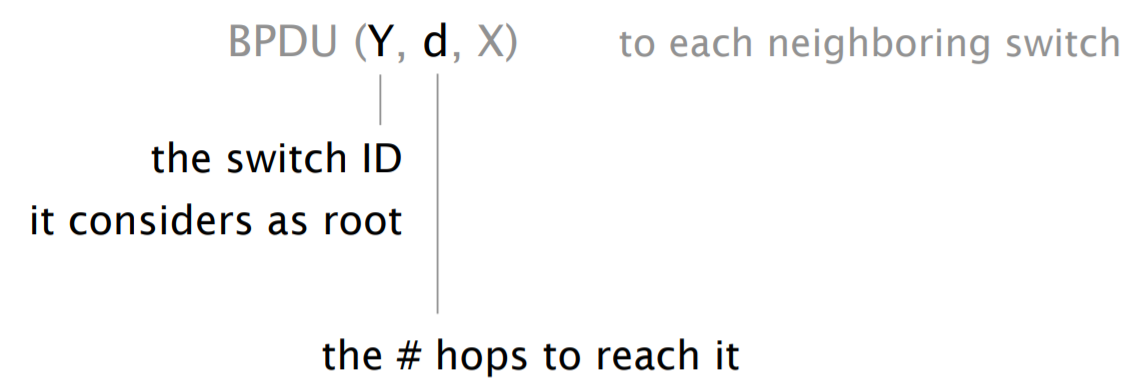
\includegraphics[width=\columnwidth]{images/Link_Layer/BPDU.png}
   		Initially: 
   		\vspace{-0.2cm}
   		\begin{itemize}[noitemsep]
   			\item Each switch proposes itself as root $\vert$ sends (X,0,X) on all its interfaces
   			\item Upon receiving (Y,d,X), checks if Y is a better root $\vert$ if so, consider Y as new root, flood updated message 
   			\item Switch compute their distance to the root, for each port $\vert$ simply add 1 to the distance received, if shorter, flood
   			\item Switches disable interfaces not on shortest-path
   		\end{itemize}
   		tie-breaking: 
   		\vspace{-0.2cm}
   		\begin{itemize}[noitemsep]
   			\item Upon receiving $\ne$ BPDUs from $\ne$ switches with $=$ cost $\rightarrow$ pick the BPDU with the lower siwtch sender ID
   			\item Upon receiving $\ne$ BPDUs from a neighboring switch $\rightarrow$ Pick the BPDU with the lowest port ID. 
   		\end{itemize}
   		To be robust, STP must react to failures: 
   		\vspace{-0.2cm}
   		\begin{itemize}[noitemsep]
   			\item Any switch, link or port can fail $\vert$ including the root switch
   			\item Root switch continuously send messages $\vert$ announcing itself as the root (1,0,1), others forward it
   			\item Failures are detected through timeout (soft state) $\vert$ if no word from root in X, times out and claims to be root 
   		\end{itemize}
   		\subsection{Virtual Local Aerea Networks VLANs}
   		The Local Area Networks we have considered so far define single broadcast domains (if one broadcasts, everyone receives it).\\
   		As the networks scales, operators like to \textbf{segment} thir LANs.\\
   		Why?
   		\begin{itemize}[noitemsep]
   			\item Improves \textbf{security} $\vert$ smaller attack surface (visibility \& injection)
   			\item Improves \textbf{performance} $\vert$ limits the overhead fo broadcast traffic 
   			\item Improves \textbf{logistics} $\vert$ separate traffic by role (staff, student,...)
   		\end{itemize} 
   		You do not want to separate your LAN physically (huge pain), but reader do it in software $\rightarrow$ \textbf{Virtual} Networks.\\
   		Definition:\\
   		A VLAN identifies a set of ports attached to one or more Ethernet Switches, forming one broadcast domain. 
   		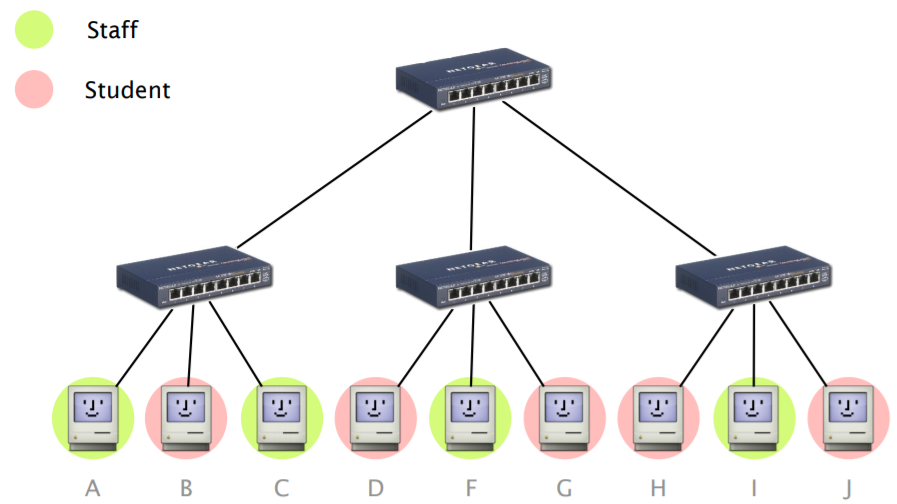
\includegraphics[width=\columnwidth]{images/Link_Layer/VLAN.png}
   		Switches need \textbf{configuration} tables telling them which VLANs are accessible via which interface.\\
   		To identify VLAN, switches add \textbf{new header} when forwarding traffic to another switch.  
   		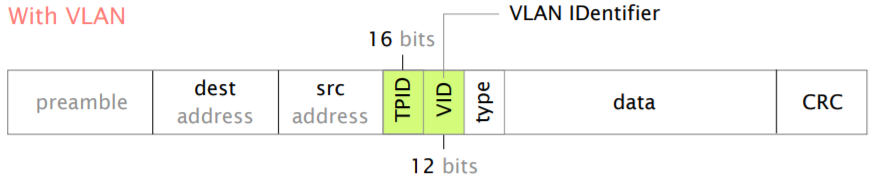
\includegraphics[width=\columnwidth]{images/Link_Layer/VLAN_header.png}
   		With VLANs, Ethernet links are divided in two sets: \textcolor{Blue}{\textbf{access}} and \textcolor{Red}{\textbf{trunks}} (inter switch) links.\\
   		Trunks carry traffic for more than one VLAN (access not), there the new header is needed! On the access links not! Communication between VLANs goes over a router!
   		Each switch runs one MAC learning algorithm for each VLAN.
   		\begin{itemize}[noitemsep]
   			\item When a switch receives a frame wit an unknown or broadcast DST.
   			\begin{itemize}
   				\item [$\rightarrow$]	it forwards it on all the ports that belong to the same VLAN
   			\end{itemize}
   		\columnbreak
   			\item  When a switch learns a SRC address on a port
   			\begin{itemize}
   				\item [$\rightarrow$] it associates it to the VLAN of this port and only uses it when forwarding frames to this VLAN	
   			\end{itemize}
   		\end{itemize}
  		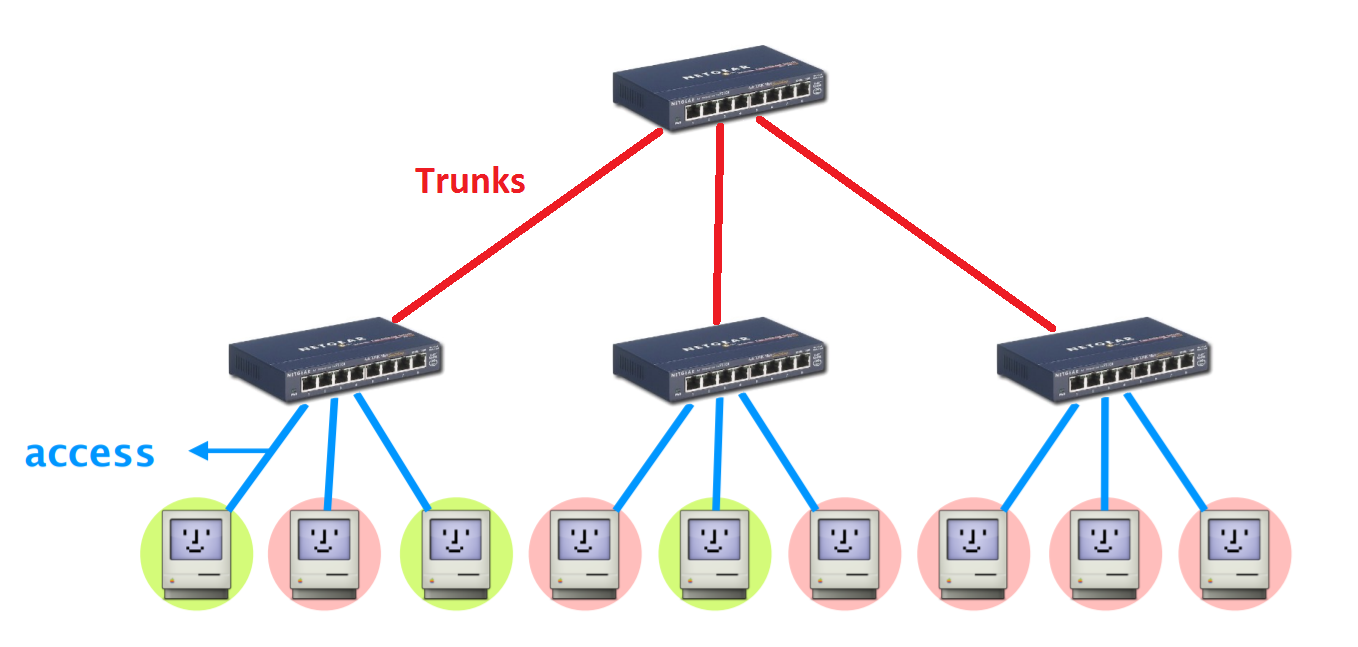
\includegraphics[width=\columnwidth]{images/Link_Layer/trunks_access.png}
   		Switches can also compute per VLAN spanning trees $\rightarrow$ distinct SPT for each VLAN! This enables better use of the network. 
   		
   		\section{The Network Layer}
   		\subsection{IP addresses}
   		IPv4 addresses are unique 32-bits number associated to a network interface (on a host, router). IP addresses are usually written using dotted-quad notation. 
   		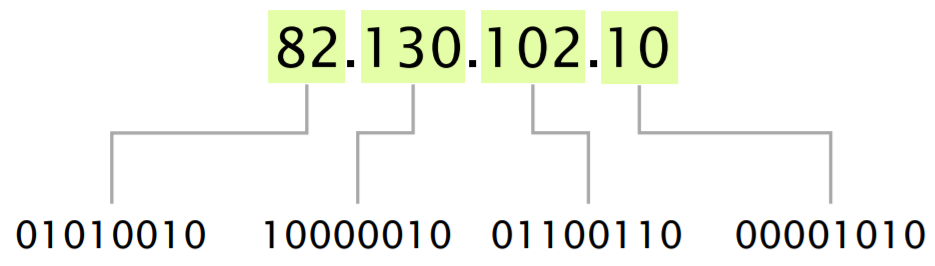
\includegraphics[width=\columnwidth]{images/Network_Layer/IP_address.png}
   		Routers forward packets based on their DST IP address. If IP addresses were assigned arbitrarily routers would require forwarding table entries for all of them!\\
   		IP addresses are hierarchical, composed of a\textcolor{Red}{ prefix (network address)} and a \textcolor{ForestGreen}{suffix (host address)}. 
   		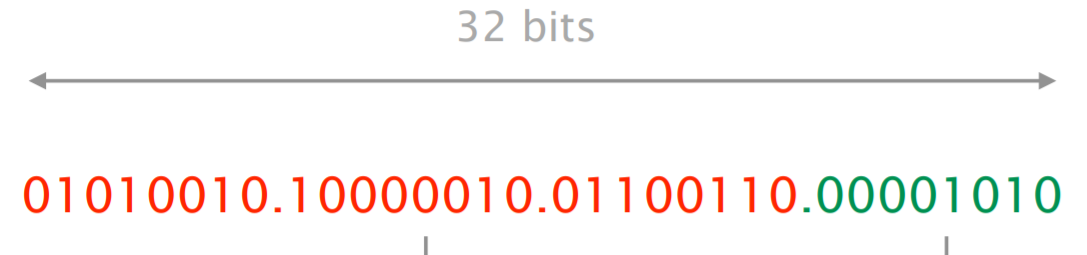
\includegraphics[width=\columnwidth]{images/Network_Layer/prefix_suffix.png}
   		Each prefix has a given length, usually written using the slash notation:\\
   		IP prefix: 82.130.102.0/\textcolor{Red}{24}$\rightarrow$ prefix length in bit\\
   		The suffix part can then be used to address the hosts of the network.\\
   		$\bullet$The \textbf{first address} of the suffix (all zeros) is used to identify the \textbf{network itself}.\\
   		$\bullet$ The \textbf{last address} of the suffix (all ones) is used ot determine the \textbf{broadcast} address.\\
   		\# of hosts $= 2^{32-\#\mathrm{\textcolor{Red}{suffix}}}-2$\\
   		Prefixes are also sometimes specified using an address and a \textbf{mask}. ANDing the address and the mask gives you the prefix. \\
   		Mask: set the number of suffix bits to one, the rest zeros (from left to right).\\
   		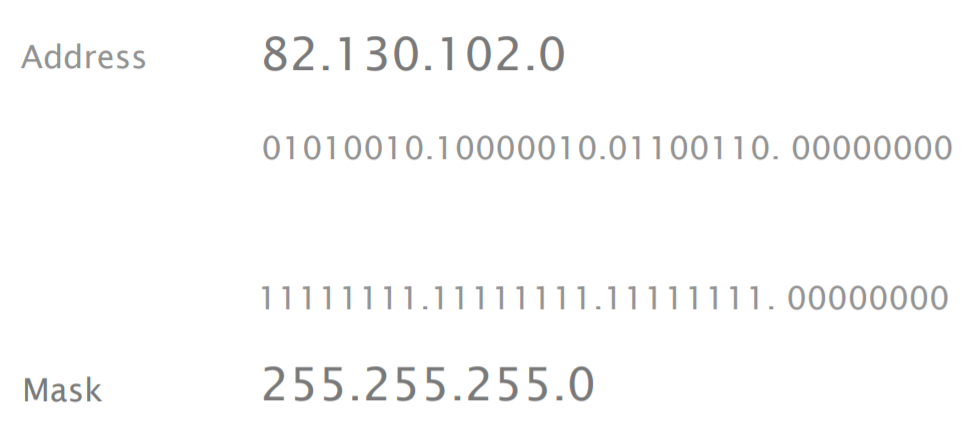
\includegraphics[width=\columnwidth]{images/Network_Layer/mask.png}
   		Routers forward IP packets based on the network part, not the host part. This enables a scaling of the forwarding table. \\
   		Originally there were only 5 fixed allocation sizes (classes) - known as classful networking. This is wasteful and leaded to IP address exhaustion.\\
   		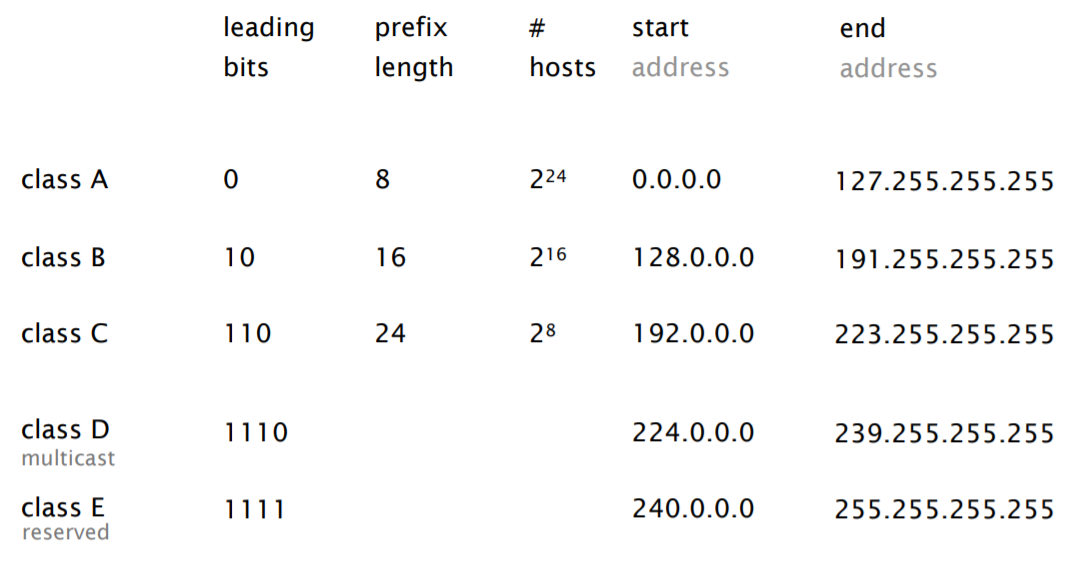
\includegraphics[width=\columnwidth]{images/Network_Layer/classes.png}
   		Problem: Class C was too small, so everybody requested B\\
   		Solution: Classless Inter-Domain Routing (CIDR) (1993)\\
   		CIDR enables flexible division between network and host addresses. 
   		\begin{itemize}[noitemsep]
   			\item CIDR must specify both, the address and the mask $\vert$ classful was communicating this in the first address bits
   			\item Masks are carried by the routing algorithms $\vert$ it is not implicitly carried in the address.  
   		\end{itemize}
   		With CIDR the maximal waste is bounded to 50\%.\\
   		Today, addresses are allocated in contiguous chunks:\\ 
   		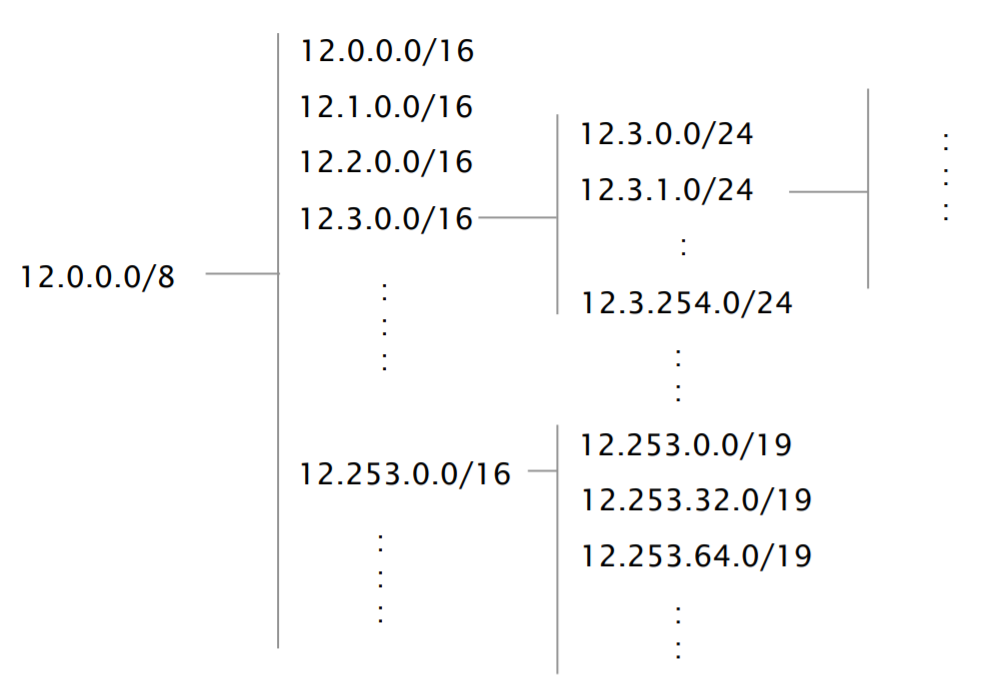
\includegraphics[width=\columnwidth]{images/Network_Layer/IP_chunk.png}
   		\pagebreak
   		
   		The allocation process of prefixes is also hierarchical:\\
   		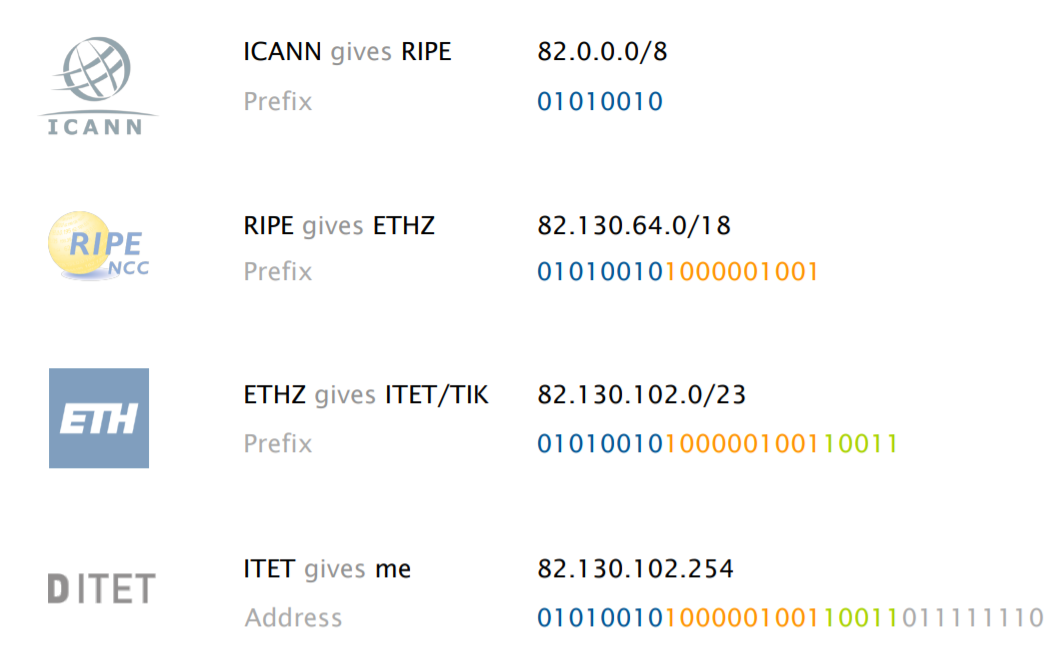
\includegraphics[width=\columnwidth]{images/Network_Layer/prefix_allocation.png}
   		
   		\subsection{IP forwarding}
   		Whats inside an IP router?:\\
   		$\bullet$ Data Plane:\\
   		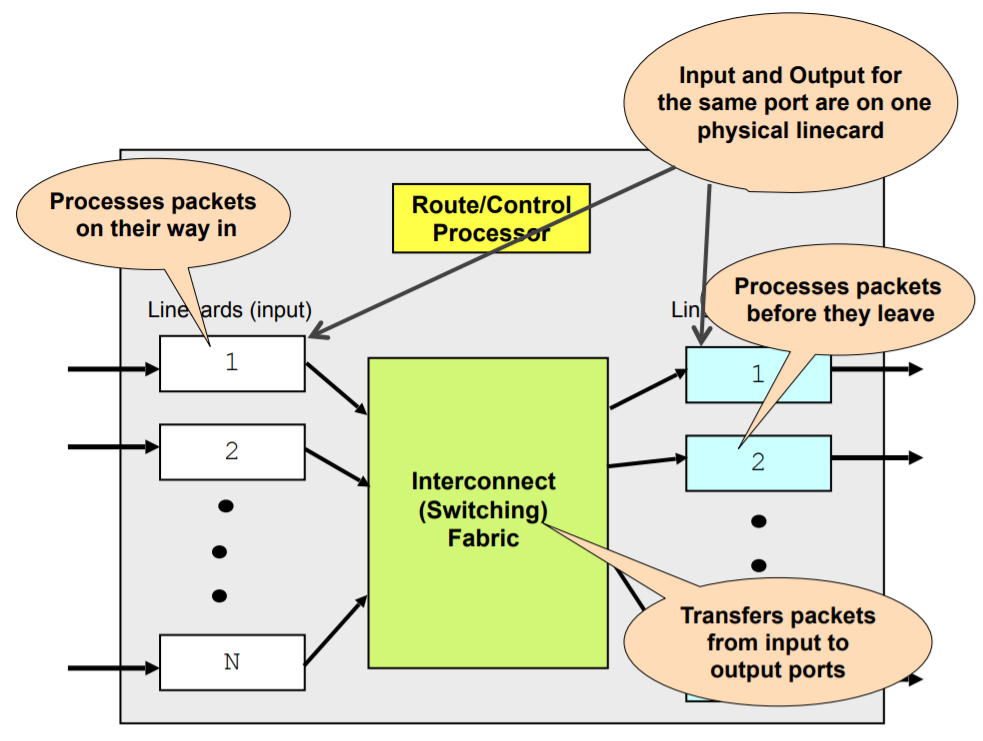
\includegraphics[width=\columnwidth]{images/Network_Layer/data_plane.png}
   		$\bullet$ Control Plane:\\
   		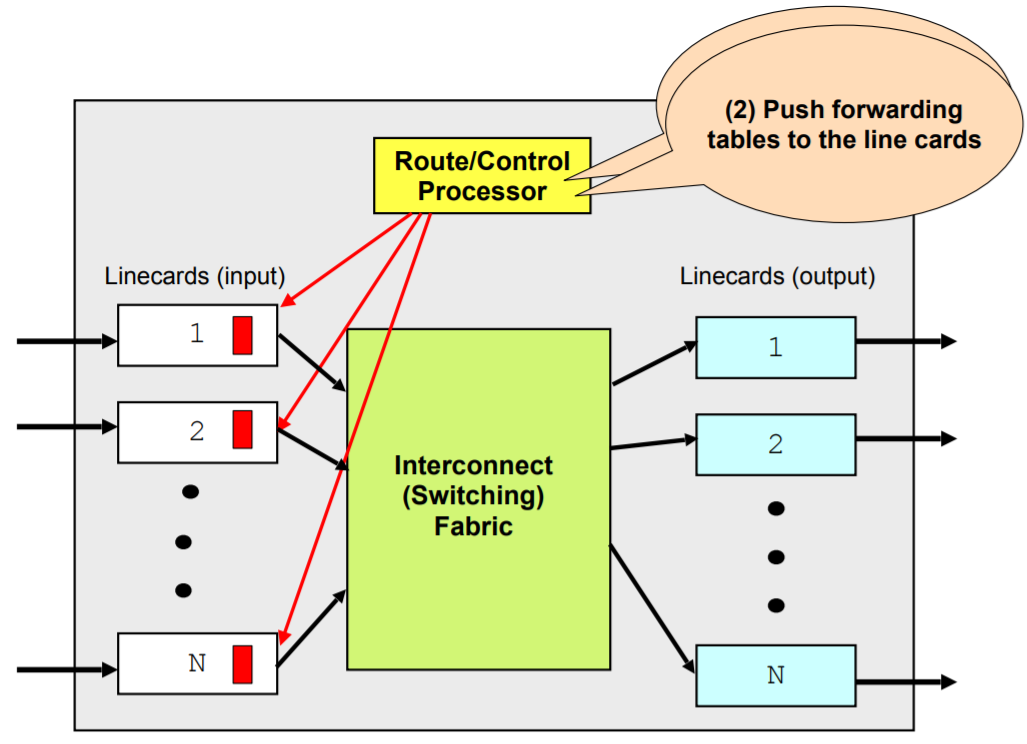
\includegraphics[width=\columnwidth]{images/Network_Layer/control_plane.png}
   		Routers maintain \textbf{forwarding entries} for each Internet prefix.\\
   		When a router receives an IP packet, it performs an IP \textbf{look up} to find the matching prefix.\\
   		CIDR makes forwarding harder, as one packet can match many IP prefixes.\\
   		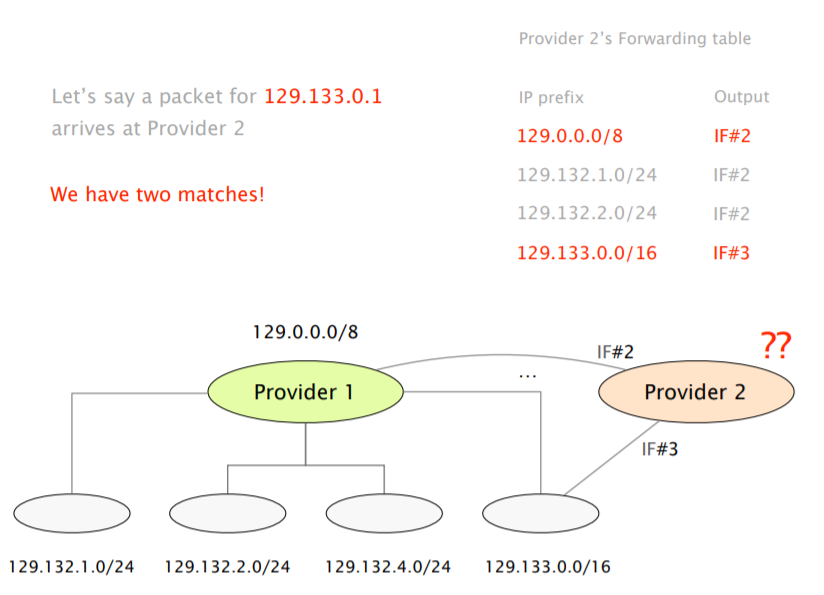
\includegraphics[width=\columnwidth]{images/Network_Layer/two_matches.png}
   		To resolve ambiguity, forwarding is done along the \textbf{most specific} prefix (IF\#3)\\
   		A child prefix can be \textbf{filtered} from the table whenever it shares the same output interface as its parent:
   		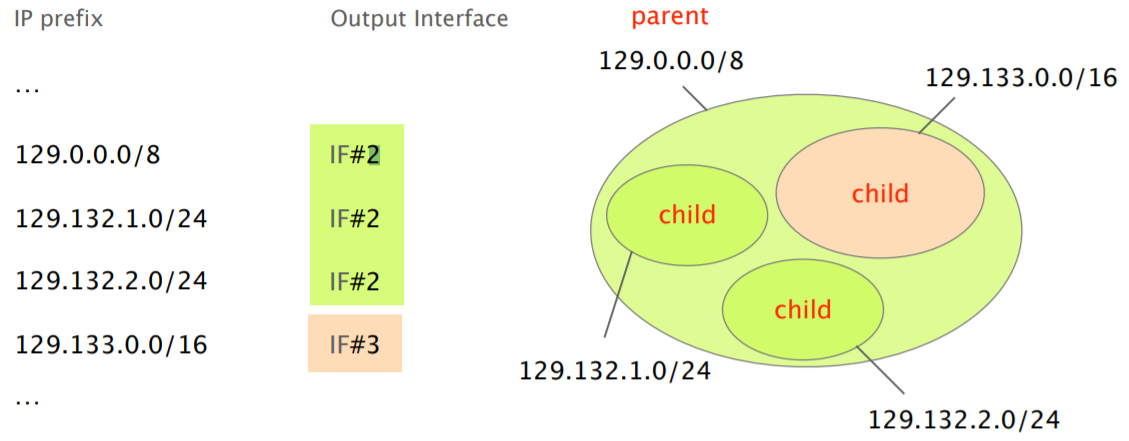
\includegraphics[width=\columnwidth]{images/Network_Layer/filtering1.png}
   		\includegraphics[width=\columnwidth]{images/Network_Layer/filtering2.png}
   		\textcolor{Red}{Exactly the same forwarding!}
   		
   		\subsection{IP header}
   	
		\end{multicols*}
	\setcounter{secnumdepth}{3}
\end{document}
